\documentclass[pdftex, 12pt, a4paper]{report}
\usepackage{tikz}
\usepackage{newtxtext, newtxmath}
\usepackage[top=2cm, bottom=2cm, left=2.5cm, right=2.5cm]{geometry}
\usepackage[hidelinks]{hyperref}
\usepackage{booktabs}
\usepackage{setspace}
\usepackage{titlesec}
\usepackage{tocloft}
\usepackage{parskip}
\usepackage{amsmath}
\usepackage{subfig}
\usepackage{minted}
\usepackage{amsfonts}
\usepackage{caption} % Required for \captionof
\usepackage[sorting=none]{biblatex}
\usepackage{listings}
\usepackage{xcolor}
\usepackage{subcaption}
\usepackage{algorithm}
\usepackage[noend]{algpseudocode}
\usepackage{amsmath}
\usepackage{xcolor}
\usepackage[utf8]{inputenc} % Enable UTF-8 encoding
\usepackage{amssymb}
\usepackage{pifont} % For checkmark and cross symbols
\usepackage{algorithmic}
\usepackage{listings}

\lstset{
    basicstyle=\small\ttfamily,
    columns=fullflexible,
    breaklines=true,
    frame=single,
    backgroundcolor=\color{white},
    keywordstyle=\color{blue},
    commentstyle=\color{gray},
    stringstyle=\color{magenta},
    showstringspaces=false
}

% Define checkmark and cross
\newcommand{\cmark}{\ding{51}} % Checkmark
\newcommand{\xmark}{\ding{55}} % Cross

\lstdefinelanguage{json}{
    basicstyle=\ttfamily\small,
    numbers=left,
    numberstyle=\tiny,
    stepnumber=1,
    numbersep=5pt,
    showstringspaces=false,
    breaklines=true,
    frame=single,
    backgroundcolor=\color{gray!10},
    stringstyle=\color{blue},
    literate=
     *{0}{{{\color{orange}0}}}{1}
      {1}{{{\color{orange}1}}}{1}
      {2}{{{\color{orange}2}}}{1}
      {3}{{{\color{orange}3}}}{1}
      {4}{{{\color{orange}4}}}{1}
      {5}{{{\color{orange}5}}}{1}
      {6}{{{\color{orange}6}}}{1}
      {7}{{{\color{orange}7}}}{1}
      {8}{{{\color{orange}8}}}{1}
      {9}{{{\color{orange}9}}}{1}
      {:}{{{\color{red}:}}}{1}
      {,}{{{\color{red},}}}{1}
      {"}{{{\color{green}"}}}{1},
}

\addbibresource{bib.bib}
\setstretch{1.5}
\setlength{\cftfigindent}{2pt}
\setlength{\cfttabindent}{2pt}
\renewcommand{\cftdotsep}{1}

% change the following
\title{\uppercase{LLM-driven code synthesis and test generation\\(Multi-Agentic Orchestration for Partial Order Estimation of Code Edits)}}
\newcommand\fypcode{H032980}
\author{Lee Zong Xun}
\date{9 April 2025}
\newcommand\degree{Bachelor of Computing in Computer Science}

\begin{document}
\makeatletter
\begin{titlepage}
\begin{center}

B.Comp. Dissertation 
\\[7cm]
\uppercase{\textbf{\large{\@title}}}

\vfill
by
\\[1cm]

\@author
\\[3cm]

Department of Computer Science \\
School of Computing \\
National University of Singapore \\
\@date

\end{center}
\end{titlepage}
\makeatother
\makeatletter
\begin{titlepage}
\begin{center}

B.Comp. Dissertation 
\\[7cm]
\uppercase{\textbf{\@title}}

\vfill

by
\\[1cm]

\@author
\\[3cm]

Department of Computer Science \\
School of Computing \\
National University of Singapore \\
\@date

\end{center}

Project No: H032980\\
Advised by: Assoc. Prof Lin Yun (SJTU)\\
Supervised by: Assoc. Prof Huang Zhiyong (NUS)
\end{titlepage}
\makeatother

\setcounter{page}{1}
\pagenumbering{roman}

\chapter*{Abstract}
\addcontentsline{toc}{chapter}{Abstract}

Large Language Models (LLMs) excel in tasks like code generation and debugging but struggle with understanding complex interdependencies in large, multifile repositories. This research aims to address these limitations by formalizing dependencies between code edits, focusing on causal-effect relationships and logical sequencing. Using multi-agent orchestration and dependency analysis, we create a framework to enhance contextual understanding and decision-making. We evaluated its effectiveness in managing complex edits and aligning with user intent, with the aim of reducing cognitive load, improving productivity, and improving AI-assisted software development.


\noindent\textbf{Subject Descriptors:}
\begin{itemize}
    \item Computing methodologies---Artificial intelligence---Natural language processing
    \item Software and its engineering---Software creation and management---Designing software---Software implementation planning
    \item Information systems---Information retrieval---Document representation
\end{itemize}

\noindent\textbf{Keywords:}\\
\hspace*{.5cm} Code Editing, Dependency Analysis, Multi-Agent Systems, Large Language Models

\noindent\textbf{Implementation Software and Hardware}:\\
\hspace*{.5cm} Pytorch, Pyright, OpenAI, Gemini, Python, Graphviz, SOC Compute Cluster

\chapter*{Acknowledgments}
\addcontentsline{toc}{chapter}{Acknowledgments}

 I would like to express my gratitude to my advisor, Assoc. Prof Lin Yun, and PhD student, Liu Chenyan, for their guidance and feedback throughout the project. Their feedback has significantly shaped my work and understanding of the subject.

\pagebreak
\addcontentsline{toc}{chapter}{Contents}
\tableofcontents

\cleardoublepage
\pagenumbering{arabic}

\chapter{Introduction}

\section{Motivation}

Large Language Models (LLMs) have demonstrated remarkable performance in code-related tasks \cite{codeium, marscode, copilot}, leveraging their extensive pre-training on programming languages and frameworks. Among these tasks, code completion has emerged as a key application, enabling LLMs to assist developers by predicting and generating code in real-time. This capability has significantly improved development efficiency and productivity, leading to the widespread adoption of AI Integrated Development Environment (IDE), such as GitHub Copilot, Cursor, and TraeAI.

While much of the current focus of code completion is on the immediate file that a developer is working on, leveraging repository-level contextual information provides additional opportunities to improve code completion. This context includes  core function definitions, configuration files, and code snippets from elsewhere in the repository that align with the developer’s current logic. By incorporating this broader context, LLMs can generate more accurate and context-aware code \cite{banerjee2024contextmatterspushingboundaries}, ultimately increasing the acceptance rate of suggestions and further enhancing coding efficiency. Although both academia and the industry have explored how to leverage repository-level information to help LLMs predict code, several practical challenges remain under-explored, particularly in real-world production environments.

% Despite these advancements, existing LLM-powered code assistants exhibit significant limitations in understanding the broader context and intent behind user edits. Their recommendations are predominantly localized, with insufficient consideration of inter-dependencies across interconnected code segments. This lack of contextual awareness becomes particularly problematic in large, multi-file projects, where such inter-dependencies are critical for maintaining code consistency and correctness. Consequently, these limitations often result in suboptimal or counterproductive suggestions, reducing the overall effectiveness of these tools.

% Addressing these challenges requires a systematic approach to enhance the contextual understanding and decision-making capabilities of LLM-based code assistants. This includes developing methods to handle complex, multi-step development tasks that demand a high-level understanding of a codebase, as well as designing mechanisms to prioritize and sequence recommendations in a manner that aligns with broader project goals and user intent. 

\newpage
\section{Objective}

Current approaches do not effectively incorporate developers’ cross-file browsing and editing behavior \cite{guan2024contextmodule}, missing valuable intent information. This research seeks to address this limitation by formalizing methods to infer, prioritize, and sequence dependencies between edits. By enhancing understanding of causal-effect relationships and edit sequencing, the objective is to empower LLM agents to:

\begin{enumerate}
    \item Anticipate user requirements by identifying context-aware dependencies.
    \item Align logically coherent and semantically consistent edit sequences with user intent.
    \item Enhance developer productivity through reliable, and context-driven recommendations.
\end{enumerate}

% Achieving these objectives will not only reduce developer cognitive load and minimize errors but also promote seamless collaboration between developers and AI systems, ultimately improving the efficiency and quality of the software development process.


\subsubsection{Formalizing Causal-Effect relationships of Edits}

Understanding these relationships is essential for developing a model that can accurately propagate changes. We will categorize and formalize various types of relationships, such as dependencies, conditional changes, and sequential modifications. This provides the foundation for further research.

\subsubsection{Derive an agentic workflow to estimate partial orders}

Orchestrating multiple agents involves assigning specialized tasks to individual agents, each responsible for specific aspects of the partial order estimation process. For instance, one agent might identify local dependencies, while another evaluates global implications across the codebase. These agents communicate iteratively, leveraging the DAG structure to refine their understanding of edit sequences. This multi-agent workflow ensures that partial orders are determined efficiently and align closely with user intent, enabling more cohesive and context-aware code recommendations.


\subsubsection{Building a Directed Acyclic Graph (DAG)}

In the graph, nodes represent individual edits, while edges denote dependencies or causal relationships. This structure allows us to systematically track how a local edit may impact other parts of the code, making it possible to propagate changes accurately. This will be crucial in visualizing and managing the propagation paths, thereby enhancing the accuracy and reliability of automated code editing.

\section{Constraints \& Assumptions}

Constraints, and assumptions impact the scope and direction of this project. Addressing these challenges is essential to achieve reliable results and to contribute novel insights to the field.

\subsubsection{Lack of a Standard Dataset and Verification Challenges}

No gold-standard dataset currently exists for propagation of code edits, and constructing a high-quality dataset is both time-intensive and resource-intensive. This process involves curating a representative set of code samples that capture a wide range of propagated edit scenarios and performing rigorous verification to ensure accuracy. Additionally, without a pre-existing standard, establishing a reliable validation process for our dataset becomes complex, requiring custom metrics and evaluations.

\subsubsection{Assumptions for Feasibility and Scope}

To ensure feasibility, we assume that our constructed dataset will adequately represent real-world propagated edits, even with some limitations in diversity and scale. While we aim to capture causal relationships accurately, certain simplifying assumptions may be applied to improve computational efficiency. In cases where precise partial ordering is challenging, heuristic-based ordering will be used to yield practical insights.

\chapter{Literature Review}

\section{Multi-Agentic Systems}

 Multi-agent LLMs has become a popular topic \cite{guo2024largelanguagemodelbased}. A large proportion of works focus on social simulation \cite{park2023generativeagentsinteractivesimulacra} and frameworks \cite{li2023camelcommunicativeagentsmind}. Based on the success of them, some
 works explore the game settings \cite{light2023avalonbenchevaluatingllmsplaying}, world wars \cite{hua2024warpeacewaragentlarge}, economy markets \cite{li2024econagentlargelanguagemodelempowered}, recommendation systems\cite{zhang2024generativeagentsrecommendation}, and pandemics \cite{Ghaffarzadegan_2024}. Others advance problem solving, focusing on reasoning of short text via multi-agent debating and discussing for different tasks in reasoning \cite{du2023improving, Xiong_2023, tang2024medagentslargelanguagemodels}, mechanics problems, paper review, knowledge graph construction \cite{ye2024isolationmultiagentsynergyimproving}, and code intelligence.

\subsection{Long Context Modeling for LLMs} 

Numerous application scenarios demand extremely long contexts, such as question answering, document and dialogue summarization, and code completion, where the inputs contain entire books and long articles. To tackle the challenge with long context tasks, two major directions have been explored as shown in (Table \ref{tab:prompting-strategies}): input reduction and window extension. \textit{Input reduction} reduces the length of the input context before feeding to downstream LLMs. Truncation approaches directly truncate the input. Retrieval Augmented Generation (RAG)  \cite{xu2024retrievalmeetslongcontext} extends this direction by retrieving the most relevant chunks through embedding similarity. However, because of low retrieval accuracy, LLMs could receive an incomplete context for solving the task, hurting performance \cite{yan2024correctiveretrievalaugmentedgeneration}. \textit{Window extension} extends the context window of LLMs via finetuning to consume the whole input. For instance, the context window increases from 1024 (GPT-2), 2048 (GPT-3), to 128k (GPT-4) \cite{openai2024gpt4technicalreport, Radford2019LanguageMA}. Moreover, the newest version of Claude-3 \cite{claude} supports 200k context windows. However, when the window becomes longer, LLMs struggle to focus on the needed information to solve the task, suffering from ineffective context utilization such as the “lost in the middle” issue \cite{liu2023lostmiddlelanguagemodels}. Recently, a few studies have employed text chunking algorithms to divide and process lengthy text inputs.
 
\subsection{Complex Task Reasoning} 
Previous works on complex reasoning have focused on decomposing the complex question into sub-questions to solve them step-by-step \cite{perez2020unsupervisedquestiondecompositionquestion}. Decomposed Prompting \cite{khot2023decomposedpromptingmodularapproach} leverages some predefined modules to classify each decomposed sub-question, then further decompose if needed. Recently, methods such as Chain-of-Thought \cite{wei2023chainofthoughtpromptingelicitsreasoning}, Least-to-Most prompting \cite{zhou2023leasttomostpromptingenablescomplex} and Pearl \cite{sun2023pearlpromptinglargelanguage} have been proposed for LLMs. 

\begin{table}[h!]
    \centering
    \resizebox{\textwidth}{!}{%
    \begin{tabular}{@{}llccccccc@{}}
        \toprule
        \textbf{Category}       & \textbf{Example Work}   & \textbf{Rec.} & \textbf{Foc.} & \textbf{No Train} & \textbf{Read} & \textbf{Agent}  & \textbf{Applicability} & \textbf{Inter.} \\ 
        \midrule
        Input Reduction         & Truncation & \xmark       & \cmark        & \cmark            & $k$           & Single          & Generic               & Low             \\
                                & RAG       & \xmark       & \cmark        & \xmark            & $n + k$       & Single          & Query-based          & Medium          \\
        \midrule
        Window Extension        & Position Interpolation  & \cmark & \xmark & \xmark & $n$ & Single & Generic & Low \\
                                & Long Context          & \cmark & \xmark & \xmark & $n$ & Single & Generic & Low \\
        \midrule
        Multi-agent LLMs        & Chain-of-Agents     & \cmark       & \cmark        & \cmark            & $n$           & Multiple        & Generic               & High            \\
        \bottomrule
    \end{tabular}
    }
    \caption{Comparison between Chain-of-Agents and prior methods for long-context tasks. Rec./Foc.:
 being able to mitigate inaccurate receptive field/long context focusing issues. Read: the number of
 tokens as model input, where n is the total input length, k is the context window limit of LLMs.
 Inter.: the interpretability of the approach. Note that RAG is ‘medium interpretable’ because of the
 re-ranked chunks.}
    \label{tab:prompting-strategies}
\end{table}

\section{Code Completion Systems}

Large Language Models (LLMs) have demonstrated impressive capabilities in code completion tasks \cite{codeium, marscode, copilot}, where they assist developers by predicting and generating new code in real-time. Much of existing research focus on leveraging repository-level contextual information to provide opportunities to improve code completion. This context includes core function definitions, configuration files, and code snippets from elsewhere in the repository that align with the developer’s current logic (Figure \ref{fig:completion}). Beyond context, a series of algorithms select relevant code snippets or comments from the current file and other sources before being filtered and assembled into the final prompt \cite{copilotx}. By incorporating these strategies, LLMs can generate more accurate and context-aware code, ultimately increasing the acceptance rate of suggestions and further enhancing coding efficiency. 

\begin{figure}
    \centering
    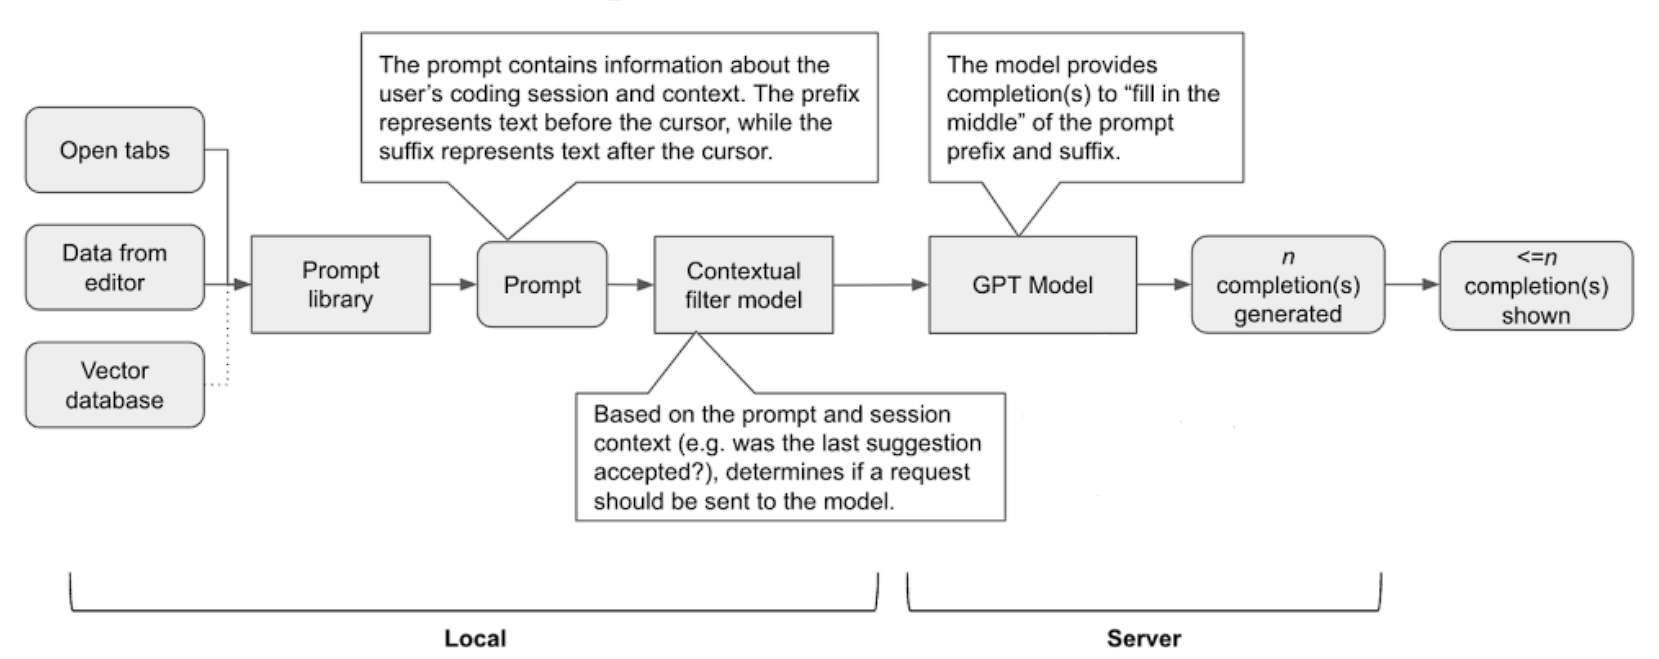
\includegraphics[width=0.8\linewidth]{fig/completion.png}
    \caption{Life of a Completion}
    \label{fig:completion}
\end{figure}

\subsection{Associated Challenges}

Several challenges remain when deploying these models in real-world environments.

\subsubsection{Limited Contextual Understanding}
While relying on the content of the file the user is working on can generate useful suggestions \cite{copilotx}, it often lacks the broader repository-level context that can be crucial for more complex tasks \cite{banerjee2024contextmatterspushingboundaries}. For instance, relevant function definitions, configuration files, or similar snippets elsewhere in the repository may not be considered, limiting the model’s ability to generate the most accurate or context-aware code.

\subsubsection{User Behavior and Intent Recognition}
Developers frequently browse and edit code across multiple files while working on a particular task. This cross-file behavior contains implicit information about the developer’s intent \cite{coeditor, coedpilot} that can be valuable for code generation. However, current code completion systems \cite{copilot, codeium, marscode} do not effectively incorporate this user behavior, resulting in suggestions that may not fully align with the developer’s immediate goals. 

\subsubsection{Efficient Retrieval of Information}
Retrieving necessary contextual information can be time-consuming and computationally expensive. For example, developers working on a large project may need relevant snippets, function signatures, or symbol definitions from different parts of the repository to guide their current task. However, real-world deployment of LLM tools introduces strict latency requirements, especially in code completion, where developers expect suggestions to appear instantly \cite{cursorai}. The challenge is to balance accuracy while keeping response times within acceptable limits.


\subsection{Methods for Better Contextual Information}

To address these challenges, recent research have integrated machine learning with dependency-aware planning to address the complexities of multi-file editing in large projects.

\subsubsection{Context-Aware Edit Representation}

Using prompting techniques and various encoding schemas, the prompt captures both the content of each edit and its surrounding context, enabling precise and contextually relevant suggestions. By leveraging Fill-in-the-Middle (FiM) \cite{bavarian2022efficienttraininglanguagemodels}, the model predicts not only the immediate next steps but also intermediate edits, thus improving its adaptability to non-linear workflows. Similarly, line-diff encoding emphasizes the differences between code versions, allowing the framework to focus on incremental changes and better understand the developer's intent.

\subsubsection{Dependency-Aware Planning}

Dependency-aware planning systems complement the process by tracking both syntactic and semantic relationships within the codebase \cite{coedpilot}. By incrementally updating dependency graphs with each edit, these systems ensure adaptive, repository-wide consistency and effectively anticipate the downstream impacts of code changes. 

\subsubsection{Interactive and Multi-Round Editing}

Human-in-the-loop frameworks (Figure \ref{fig:trae}) make code completion more intuitive by incorporating user inputs and feedback into the editing process. These frameworks dynamically adapt to prior changes, leveraging a multi-stage analysis to identify the files and lines most likely to require updates. This approach allows developers to guide the model's recommendations, ensuring that subsequent edits are contextually relevant and aligned with user intent. By fostering an interactive and collaborative editing experience, human-in-the-loop frameworks \cite{marscode, copilot, cursorai} simplify complex code completion tasks and enhance overall developer productivity.

\subsubsection{Heuristic-Based Approaches}

By applying rule-based strategies that streamline dependency management and refine edit locations, these approaches prioritize changes in files or functions closely related, syntactically or functionally, to the original edit, reducing redundant processing. Common heuristics \cite{coeditor, coedpilot} include proximity-based prioritization, which applies edits within syntactically related areas, and "hotspot" detection, focusing on frequently modified sections of code. By integrating these heuristics, systems can more efficiently direct computational resources to areas with higher propagation likelihood. This combination allows heuristic methods to handle both predictable, pattern-based changes and complex, adaptive editing scenarios.

\vspace{1cm}

\begin{figure}
    \centering
    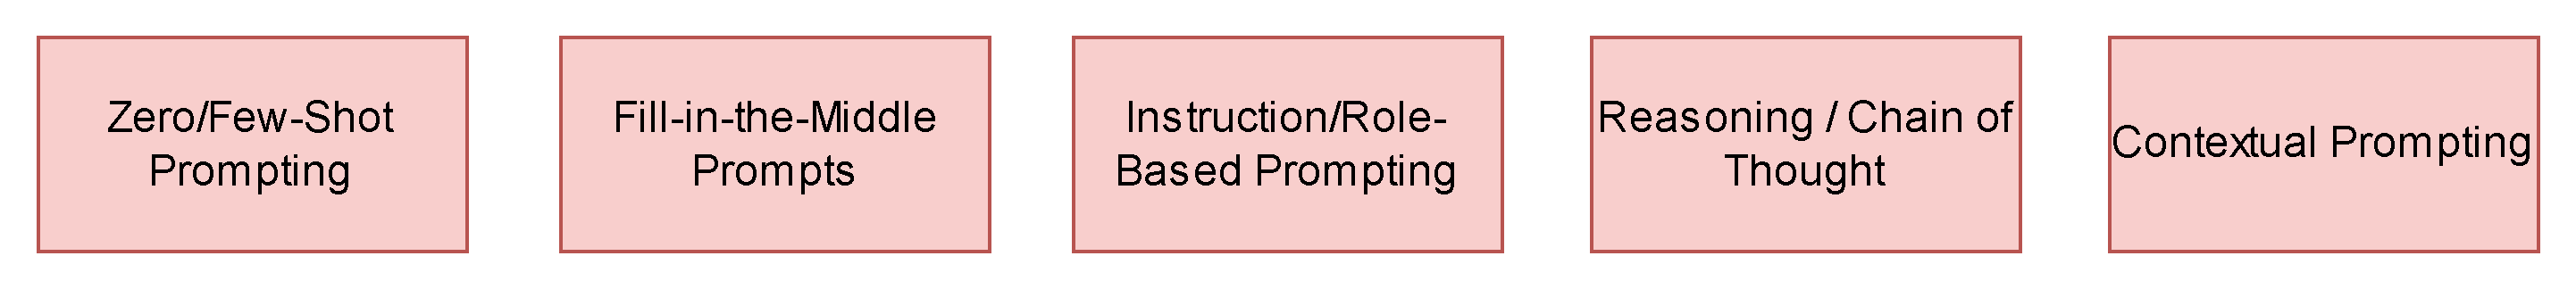
\includegraphics[width=0.8\linewidth]{fig/prompt_strats.png}
    \caption{Various prominent prompting strategies}
    \label{fig:prompt}
\end{figure}

\begin{figure}[h]
    \centering
    % First Image
    \begin{minipage}[t]{0.8\textwidth}
        \centering
        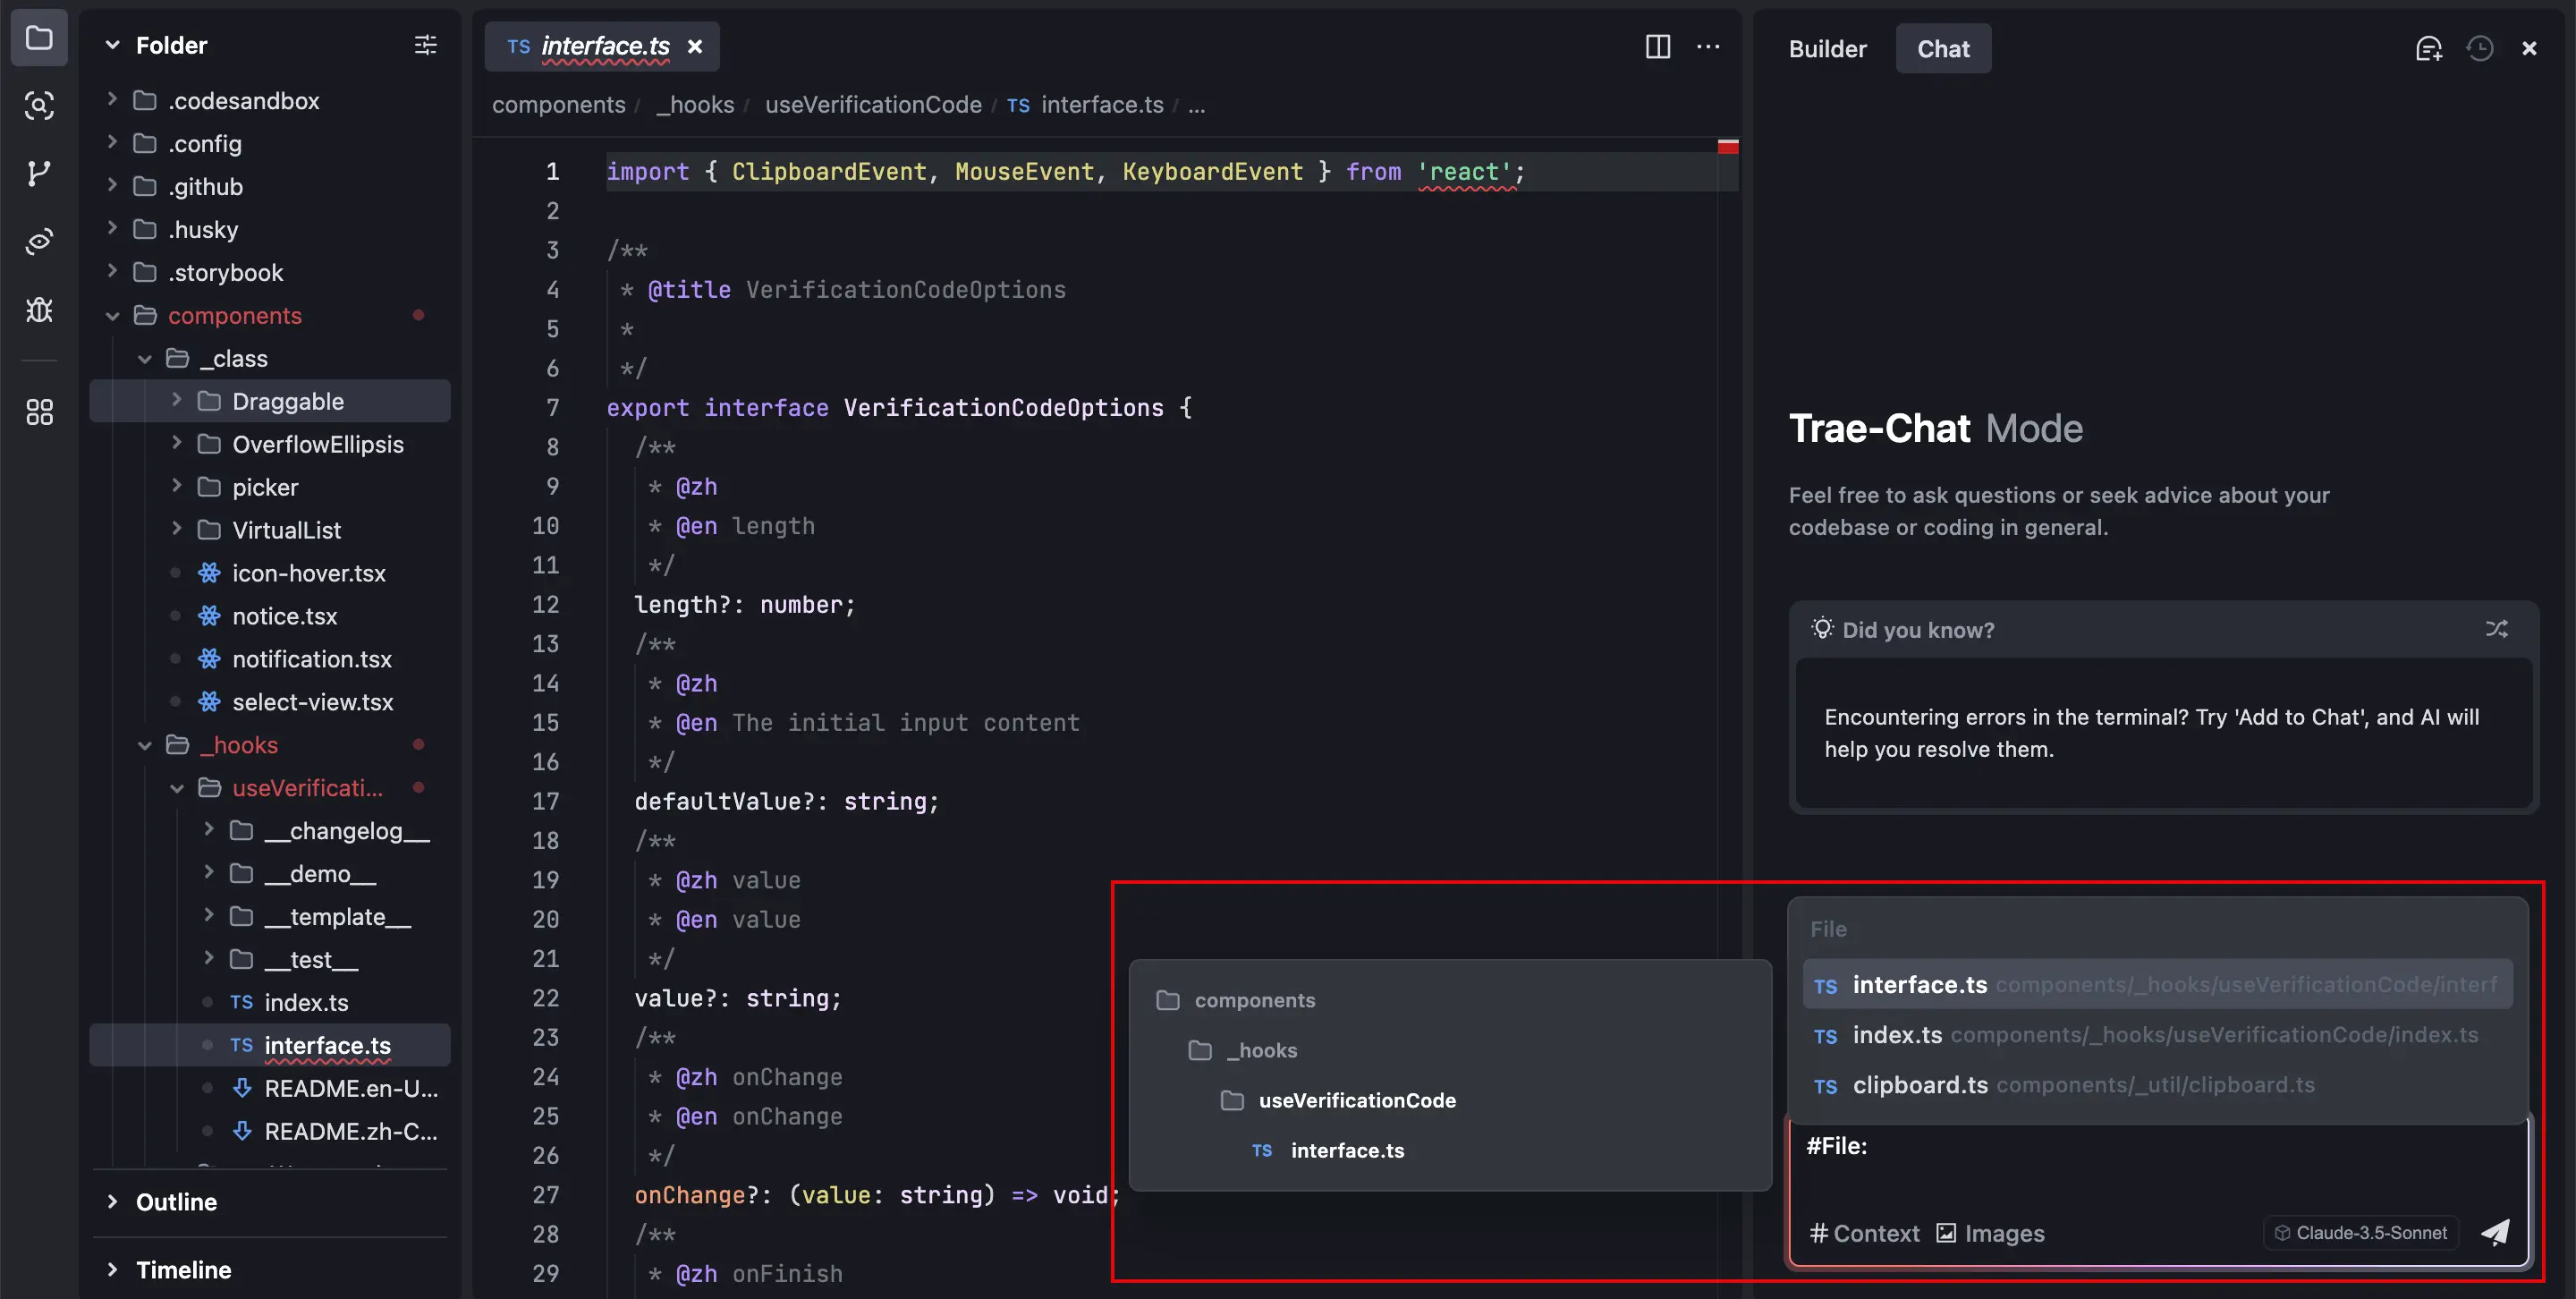
\includegraphics[width=1\linewidth]{fig/trae-1.png} % Replace with your image file
        \caption*{(a) Select relevant files as context for multi-file edits.} % Caption without label
        \vspace{0.5cm}
    \end{minipage}
    \begin{minipage}[t]{0.8\textwidth}
        \centering
        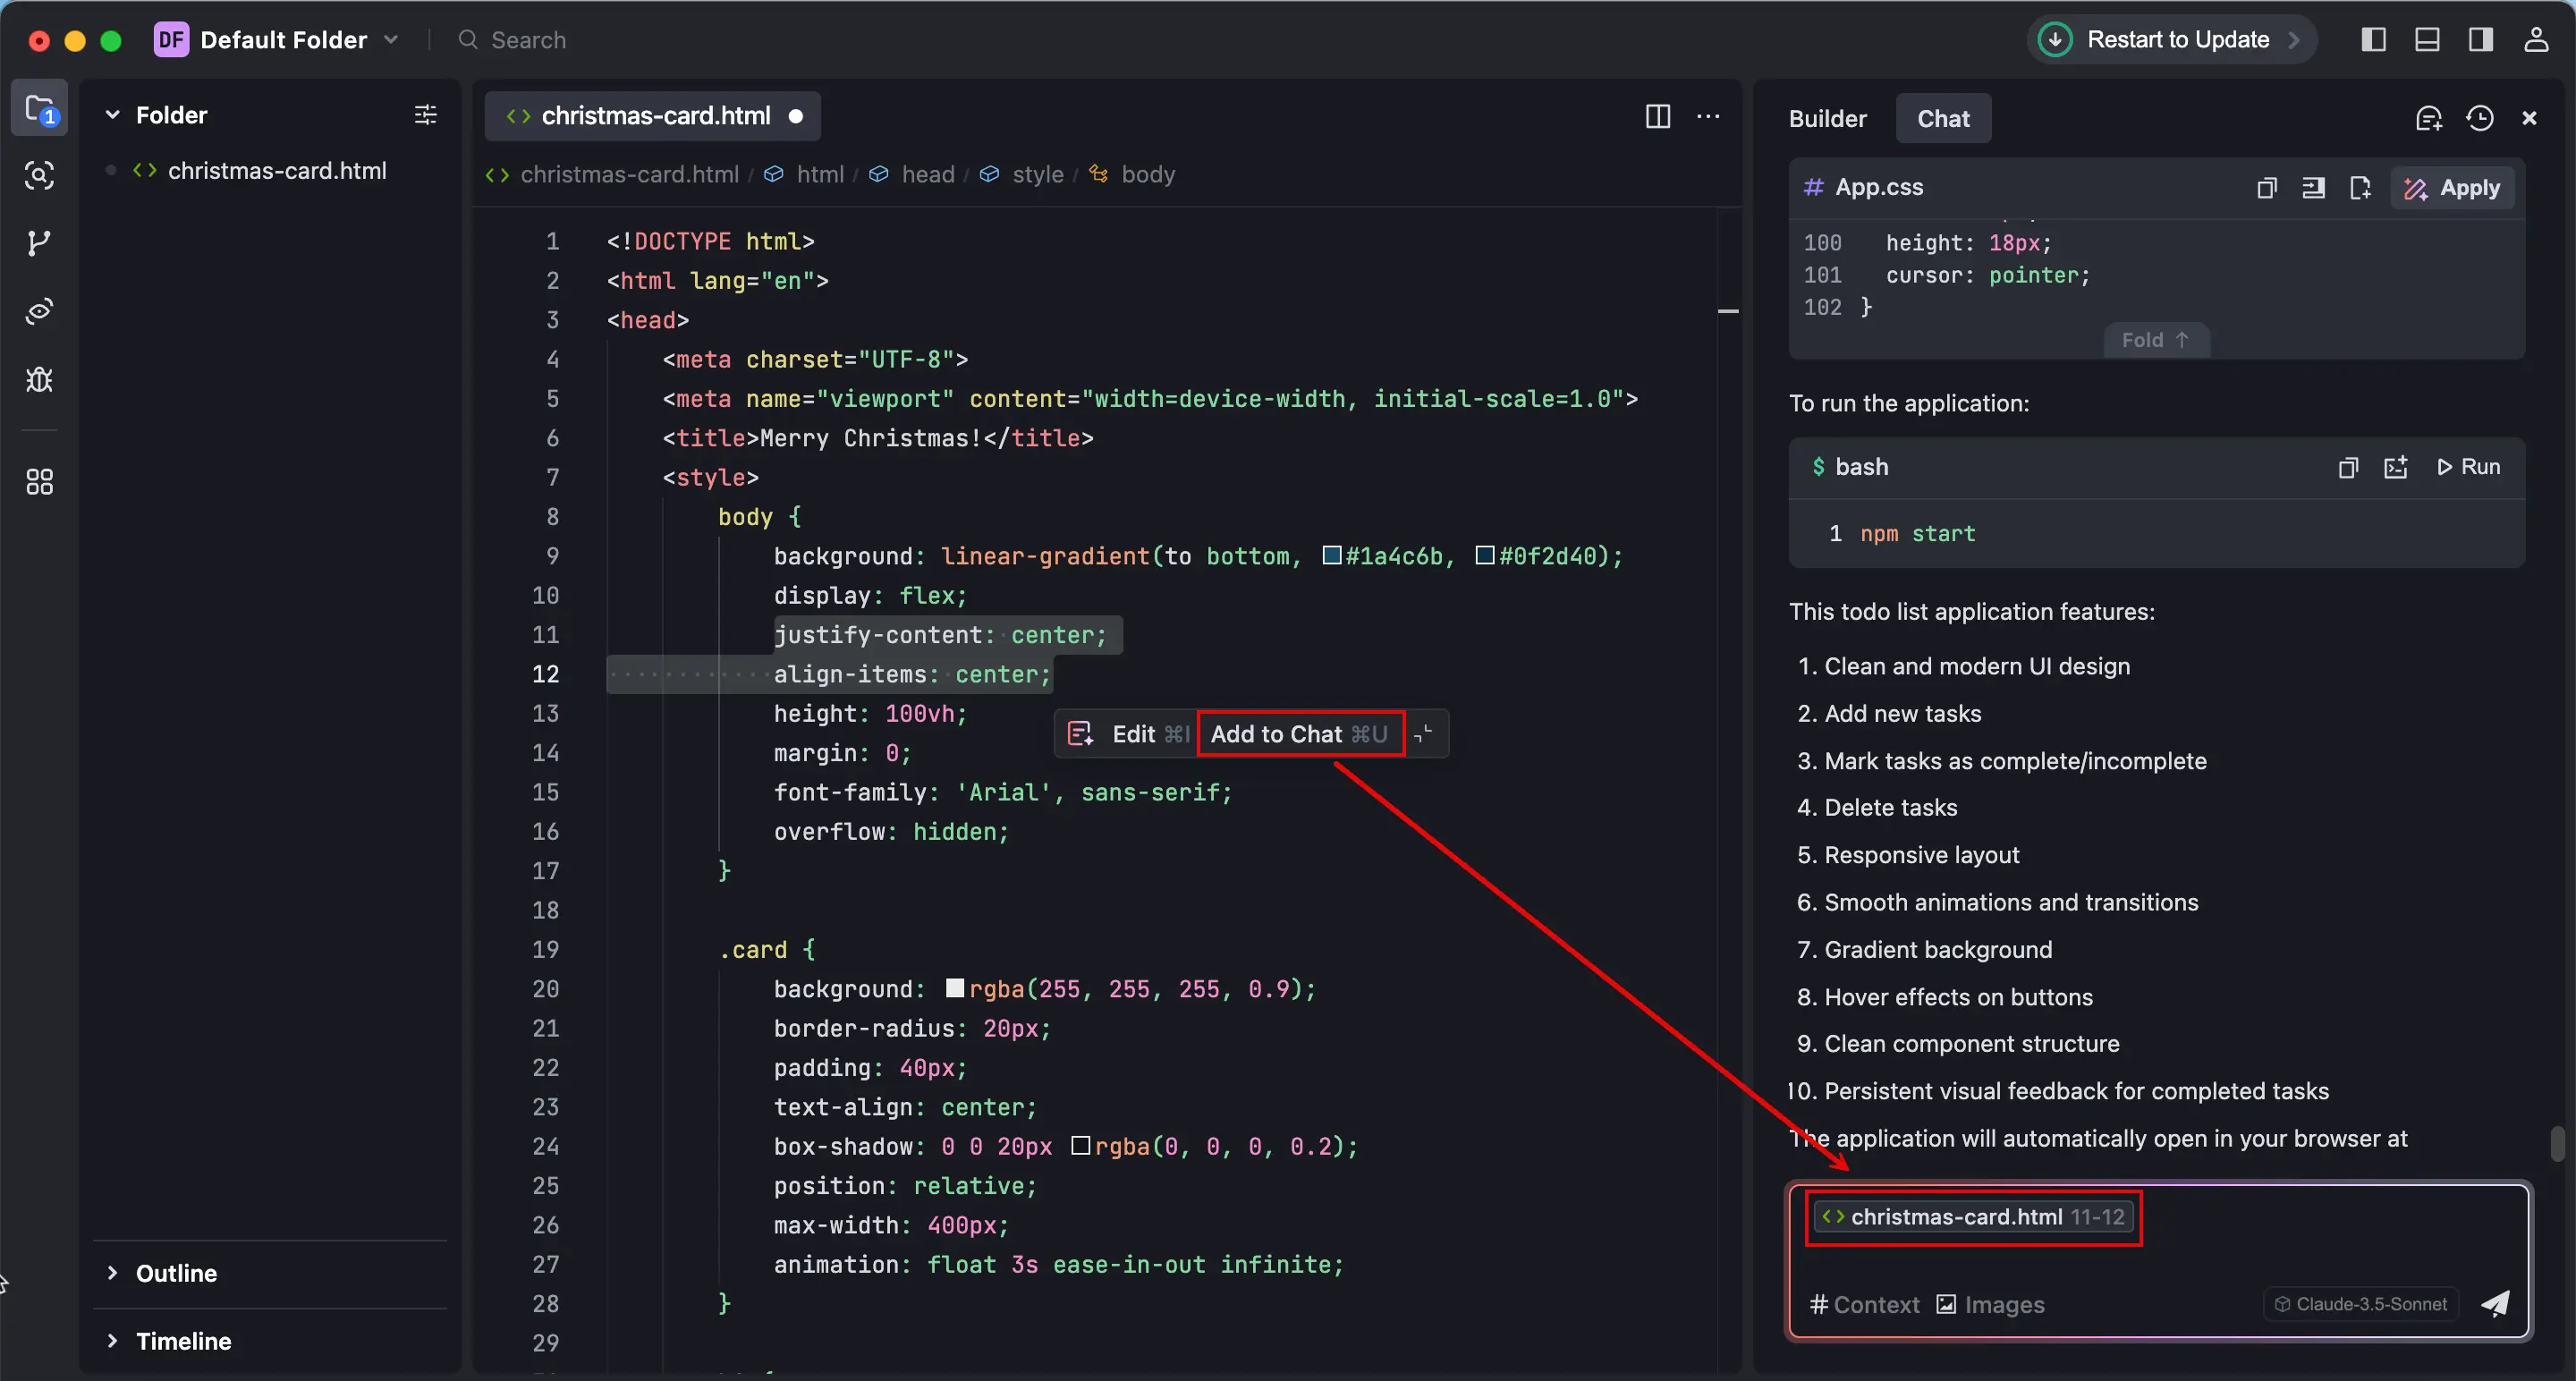
\includegraphics[width=1\linewidth]{fig/trae-2.png} % Replace with your image file
        \caption*{(b) Option to add inline code as context to chat bot.} % Caption without label
    \end{minipage}
    % Overall Caption
    \caption{Human-in-the-Loop Design in AI IDE, Trae AI.}
    \label{fig:trae}
\end{figure}


\chapter{Methodology}

\section{Problem Formulation}

We formally define the problem of determining the partial ordering of code edits within a set, denoted as \(\mathbf{H}\). Given two elements \( h_i, h_j \in \mathbf{H} \), we aim to establish the relationship between these edits in terms of their sequence or independence. This relationship is defined by a function \( f(h_i, h_j) \) that categorizes the interactions between pairs of edits as follows:
\[
f(h_i, h_j) =
\begin{cases}
    h_i \rightarrow h_j, & \text{if } h_i \text{ must occur before } h_j \\
    h_i \leftarrow h_j, & \text{if } h_j \text{ must occur before } h_i \\
    h_i \leftrightarrow h_j, & \text{if either } h_i \text{ or } h_j \text{ can occur first (no strict order)} \\
    h_i \times h_j, & \text{if there is no sequential relationship between } h_i \text{ and } h_j
\end{cases}
\]

where \(0 \leq i, j \leq n\), and \(n\) represents the total number of edits within the set \(\mathbf{H}\).

This formulation allows us to capture a range of dependencies or independencies among edits within the codebase, enabling the construction of directed acyclic graphs (DAGs) to map out the sequential relationships among edits. By applying this formulation, we can better understand and predict the propagation paths of code changes within complex systems.

\newpage
\section{Partial Order Reduction}
\label{sec:por}

The number of possible transition orderings grows exponentially (Figure \ref{fig:partial-order}). To efficiently determine the partial ordering of code edits, we used \textit{Partial Order Reduction} \cite{cirisci2022pragmaticapproachstatefulpartial} to prune any unnecessary interleaving of \textbf{independent} edits while ensuring all critical relationships are evaluated.

\begin{figure}
    \centering
    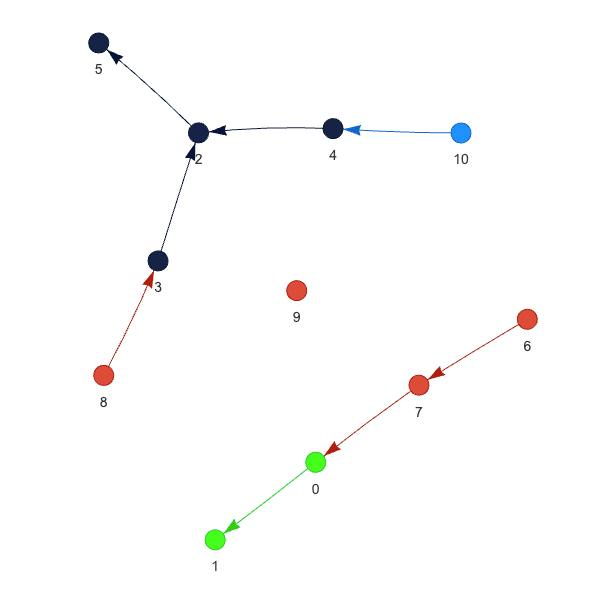
\includegraphics[width=0.5\linewidth]{fig/partial-orders.png}
    \caption{For a commit comprising 11 edits with the dependencies specified above, there are initially 13,860 possible sequences. By applying partial-order reduction, this figure drops to only 36, reflecting a 99\% decrease in the overall search space.}
    \label{fig:partial-order}
\end{figure}

\subsection{Key Components}

\textbf{Independence}: Let \( S \) represent the set of system states and \( T \subseteq S \times S \) represent the set of transitions (or actions). Two transitions \( t_1, t_2 \in T \) are considered \textit{independent} if the following conditions hold:
\begin{enumerate}
    \item \textbf{Commutativity}: The order of execution does not affect the system's state:
    \[
    t_1(s) \xrightarrow{t_2} s' \iff t_2(s) \xrightarrow{t_1} s'
    \]
    where \( t_1(s) \) represents the state resulting from applying \( t_1 \) to state \( s \).
    \item \textbf{Non-interference}: Execution of one transition does not disable the other:
    \[
    t_1 \text{ is enabled in state } s \implies t_2 \text{ is also enabled in } t_1(s).
    \]
\end{enumerate}

\textbf{Dependency}: Two transitions \( t_1, t_2 \) are \textit{dependent} if they do not satisfy the independence conditions. Dependency implies that the order of execution can affect the system state. 

\textbf{Equivalence Classes of Executions}: Define an equivalence relation \( \sim \) over the set of executions based on their observable behavior. Two executions \( \sigma_1 \) and \( \sigma_2 \) are equivalent if they differ only in the order of independent transitions:
\[
\sigma_1 \sim \sigma_2 \iff \text{same final state and equivalent under reordering of independent transitions.}
\]

\textbf{Reduction Criterion}: For a given state \( s \), a reduced set of transitions \( T_{\text{red}}(s) \subseteq T \) is selected such that every equivalence class of executions contains at least one representative path that is explored. This ensures \textit{state space preservation}:
\[
\forall t \in T, \exists t' \in T_{\text{red}}(s): \quad t \sim t'.
\]
\subsection{Workflow}

Given a system \( (S, T, s_0) \), where \( S \) is the set of states, \( T \) is the set of transitions, and \( s_0 \) is the initial state:
\begin{enumerate}
    \item \textbf{Dependency Analysis:} Compute the dependency relation \( \mathcal{D} \subseteq T \times T \) based on independence criteria.
    \item \textbf{Ample Set Selection:} For each state \( s \), select a subset of transitions \( \text{Ample}(s) \subseteq T \) such that:
    \begin{itemize}
        \item \textit{Enabledness}: \( \text{Ample}(s) \) includes only transitions enabled in \( s \).
        \item \textit{Dependency Coverage}: If a transition $t \notin Ample(s)$ is dependent on a transition in $Ample(s)$, $t$ must be eventually explored through the reduced state space.
        \item \textit{Cycle Freedom}: The reduced state space must remain acyclic under certain conditions.
    \end{itemize}
    \item \textbf{State Exploration:} Explore only the transitions in \( \text{Ample}(s) \) for each state \( s \).
    \item \textbf{Pruning:} Avoid re-exploring states that are equivalent under the equivalence relation \( \sim \).
\end{enumerate}

\subsection{Preservation Properties}
Partial Order Reduction guarantees\footnote{The full proof of the liveness and safety properties can be found in Appendix A} the preservation of certain properties in the reduced state space:
\begin{itemize}
    \item \textbf{Safety:} If the original system satisfies a safety property (e.g., no deadlock), the reduced system will also satisfy it.
    \item \textbf{Liveness:} If the original system satisfies liveness properties (e.g., progress), the reduced system will as well.
\end{itemize}

Formally:
\[
\forall \phi \in \mathcal{P}: \quad (S, T, s_0) \models \phi \iff (S_{\text{red}}, T_{\text{red}}, s_0) \models \phi
\]
where \( \mathcal{P} \) is the set of properties being verified.

\subsection{Directed Acyclic Graph}
The dependency relationships derived through POR can be represented as a Directed Acyclic Graph: 
\begin{itemize}
    \item \textbf{Nodes}: Represent individual edits $h_i \in \mathbf{H}$
    \item \textbf{Edges}: Represent transitions $h_i \rightarrow h_j$, indicating that $h_i$ must occur before $h_j$
\end{itemize}

\section{Dependency Analysis}
We present the observations and work to formalize the various types of dependencies.

\subsection{Observations}

The following are key observations (examples provided in Figure \ref{fig:observations}):

\begin{enumerate}
    \item A single edit region may contain multiple edit semantics, which may require multiple rounds of parsing before full processing.
    \item The order of edits should be arranged based on their dependencies to ensure correct sequencing.
    \item Independent edits can be applied concurrently with no regards to consequences.
    \item Edits within the same code block are more likely to occur sequentially due to their local dependencies and proximity.
    \item Inter-file dependencies are often mediated through shared components (e.g., imports, global variables, or shared libraries).
\end{enumerate}


\begin{figure}%
    \centering
    \subfloat[\centering One edit region may contain multiple edit semantic, that may be visited twice]{{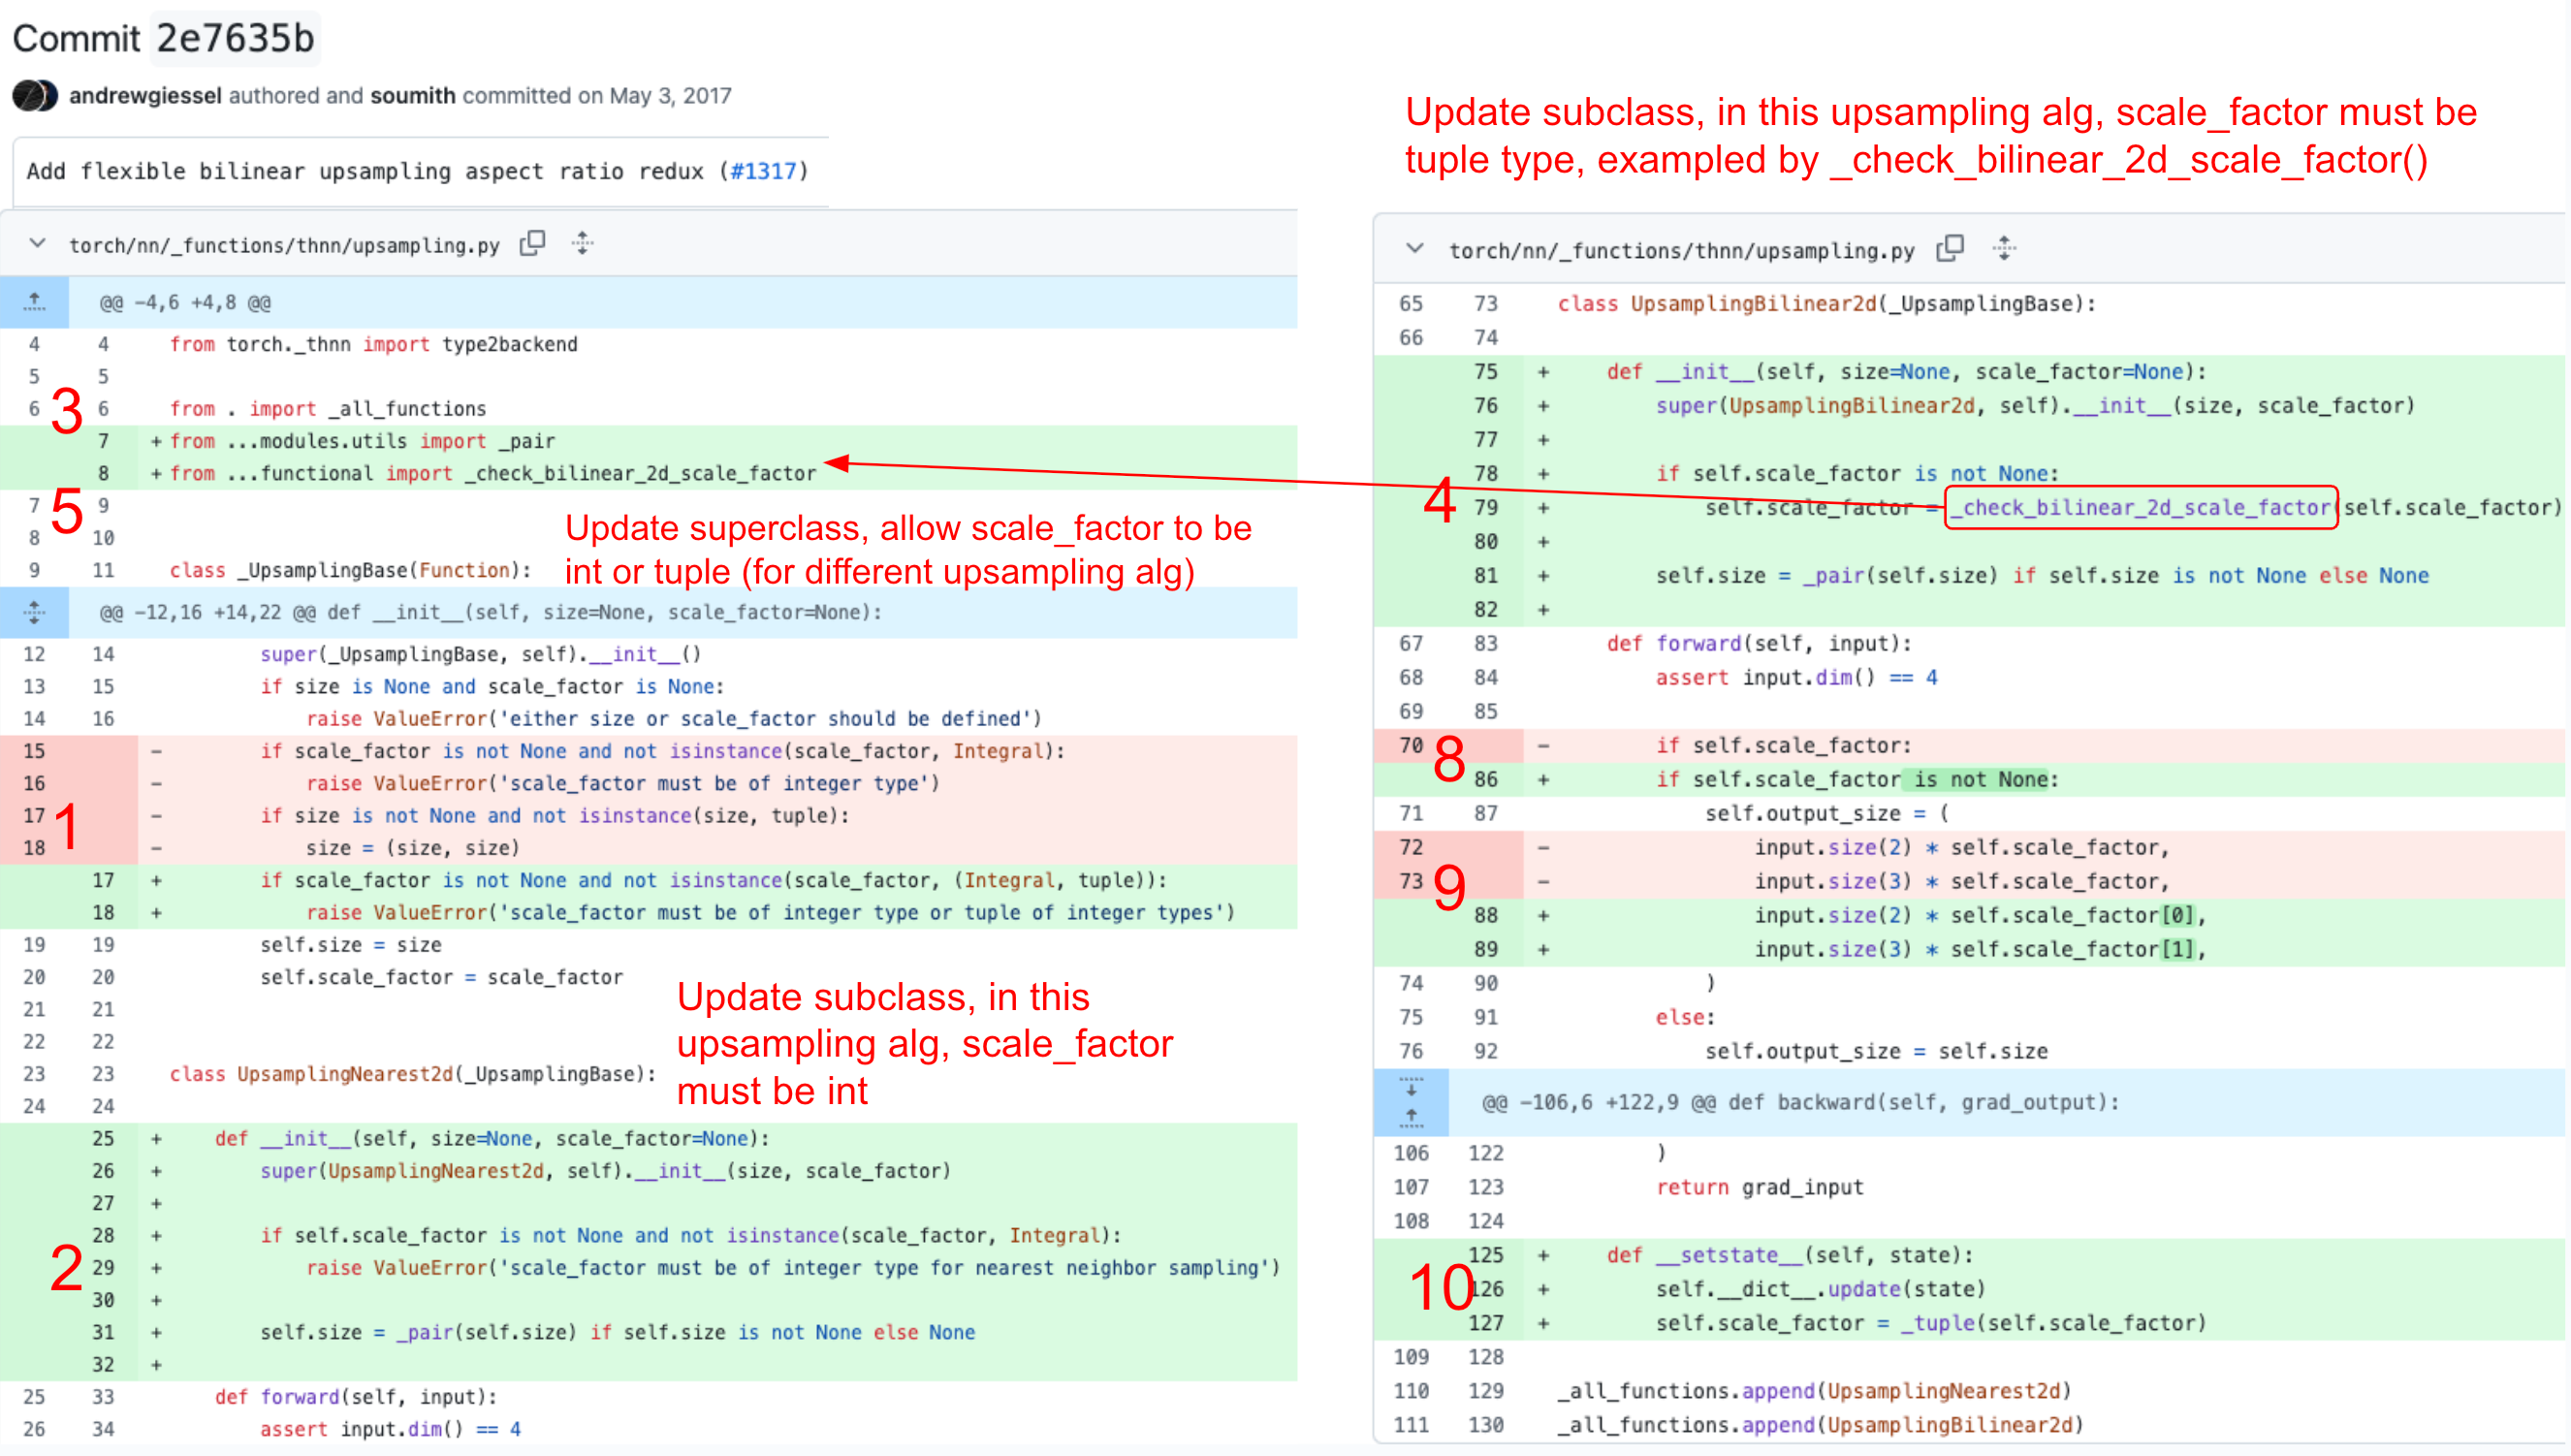
\includegraphics[width=9cm]{fig/obs_1.1.png} }}%
    \qquad
    \subfloat[\centering Arrange edit order by their dependency]{{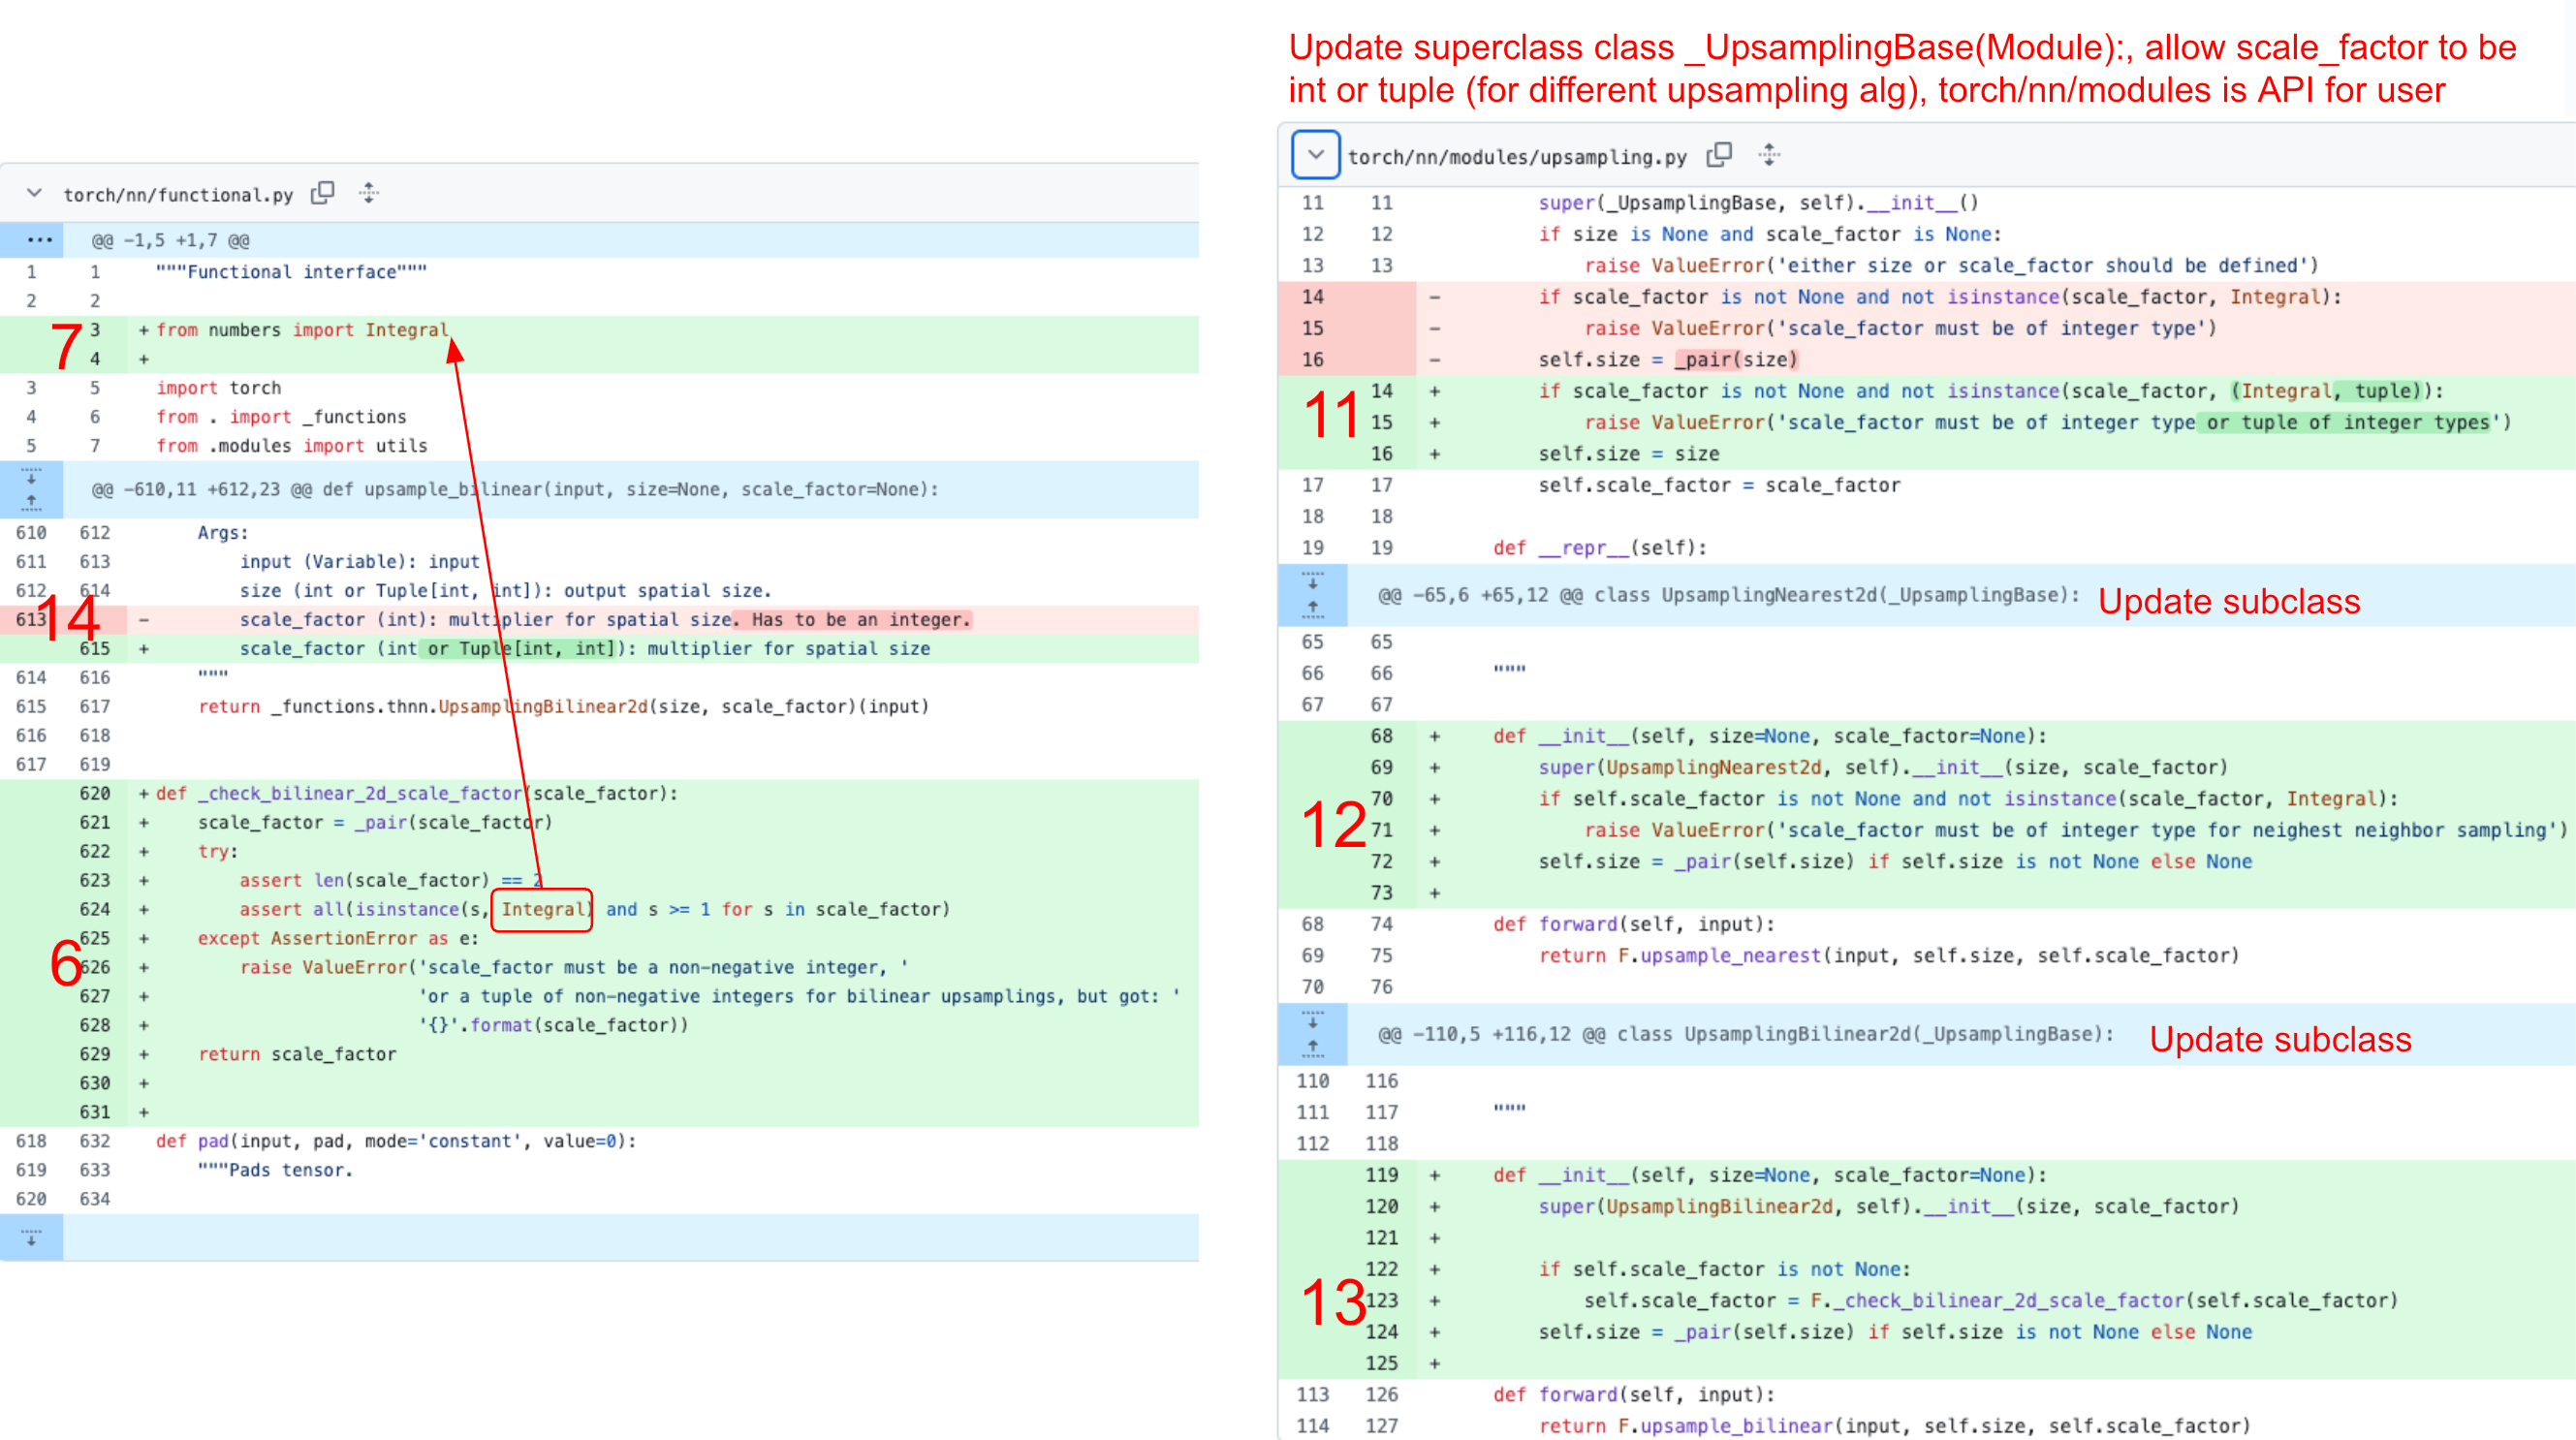
\includegraphics[width=9cm]{fig/obs_1.2.png} }}%
    \qquad
    \subfloat[\centering Parallelism between similar edit compositions]{{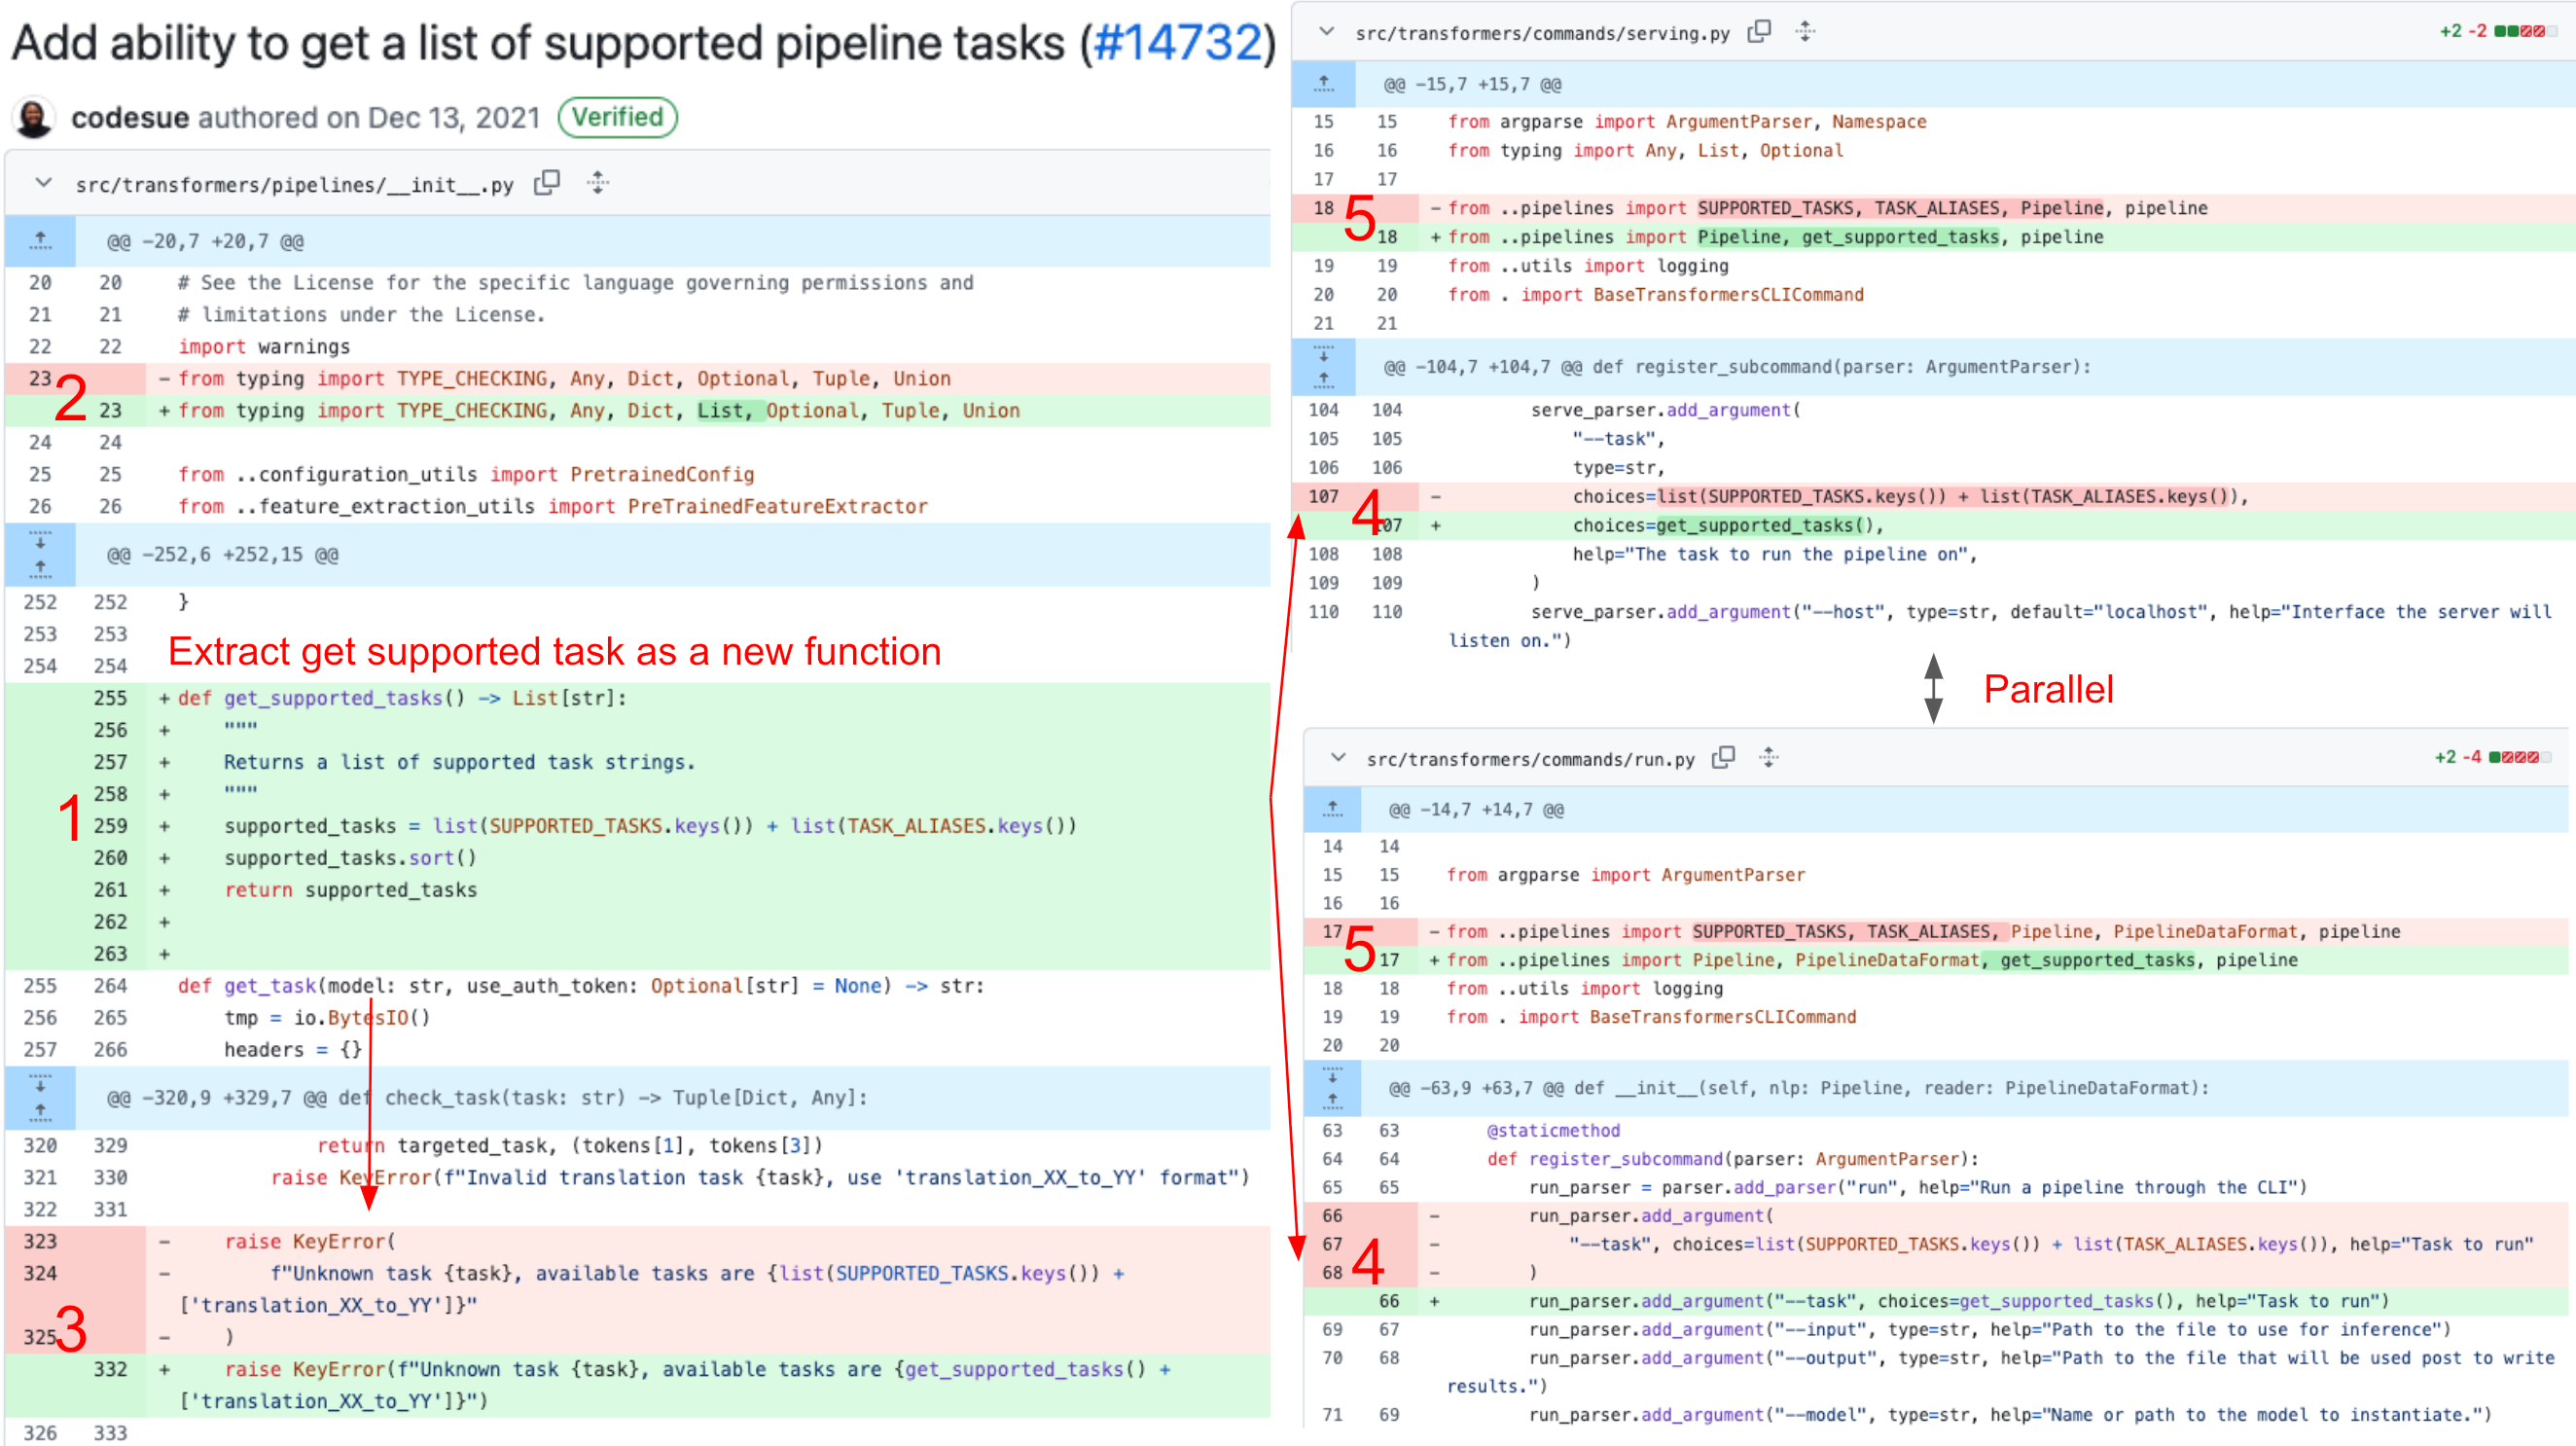
\includegraphics[width=9cm]{fig/obs_1.3.png} }}%
    \qquad
    \subfloat[\centering Edits in the same block are more likely to happen in sequential order]{{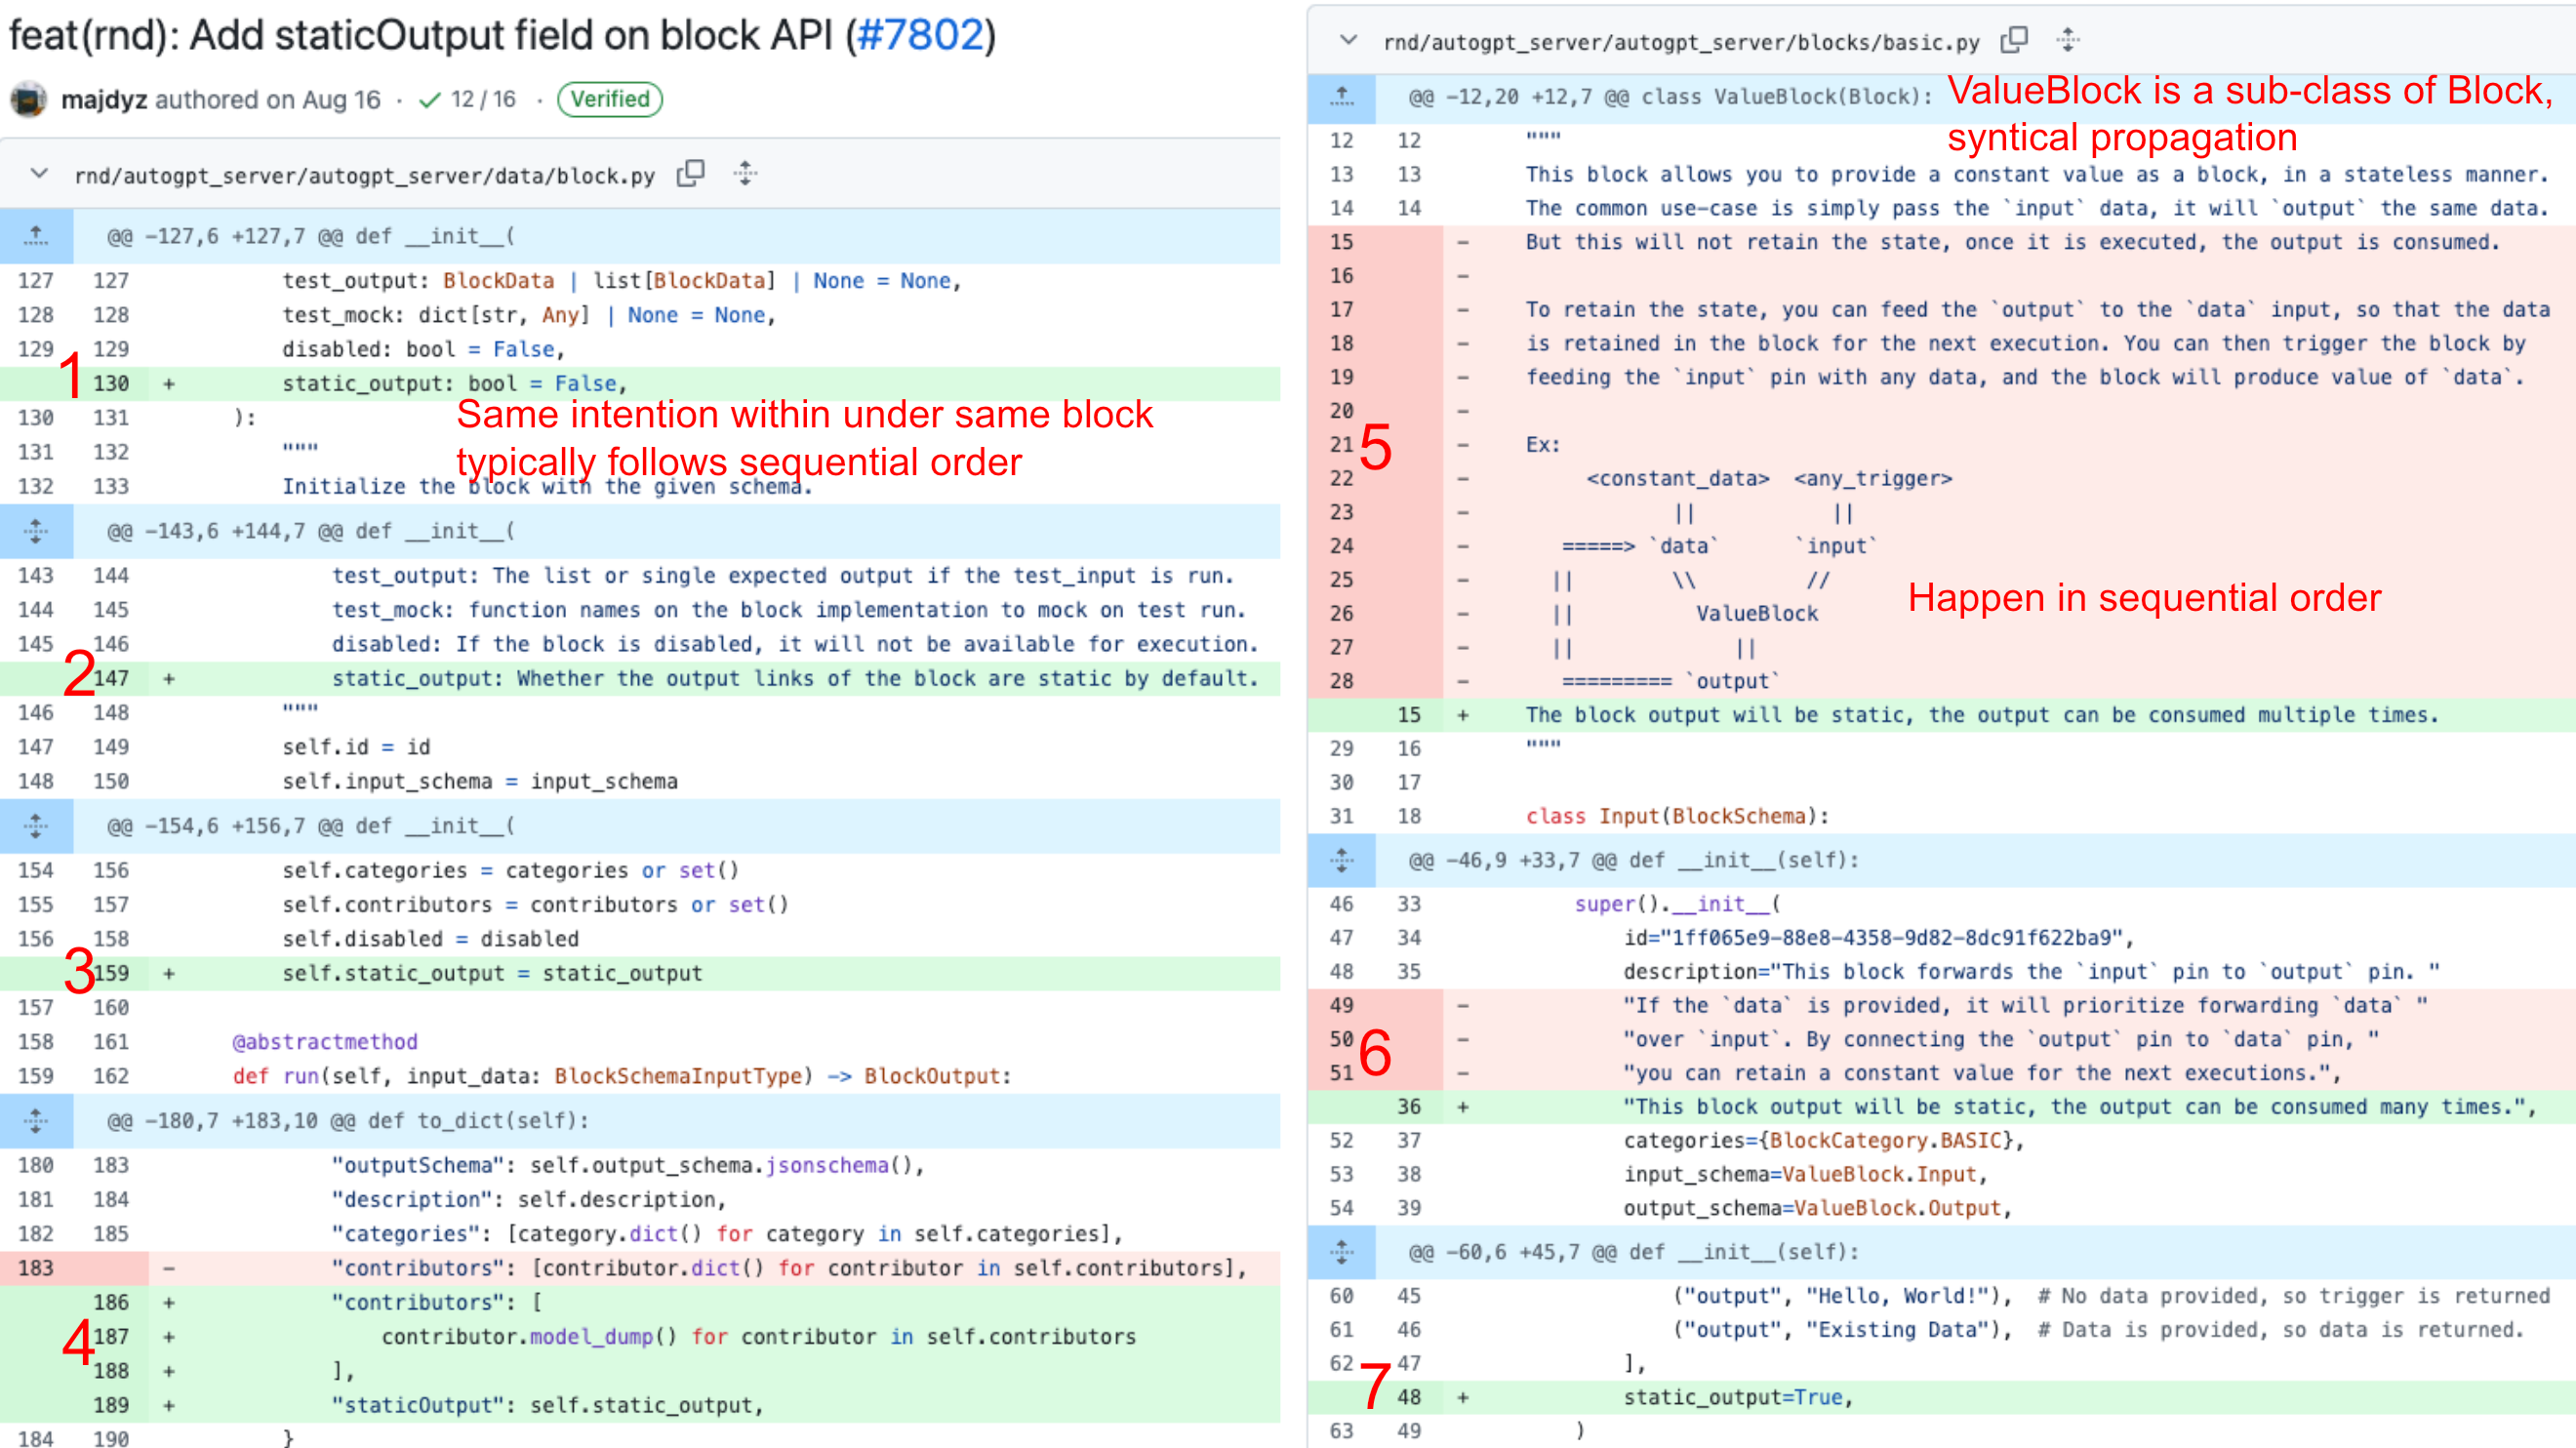
\includegraphics[width=9cm]{fig/obs_1.4.png} }}%
    \caption{Observations}%
    \label{fig:observations}%
\end{figure}


% \begin{figure}
%     \centering
%     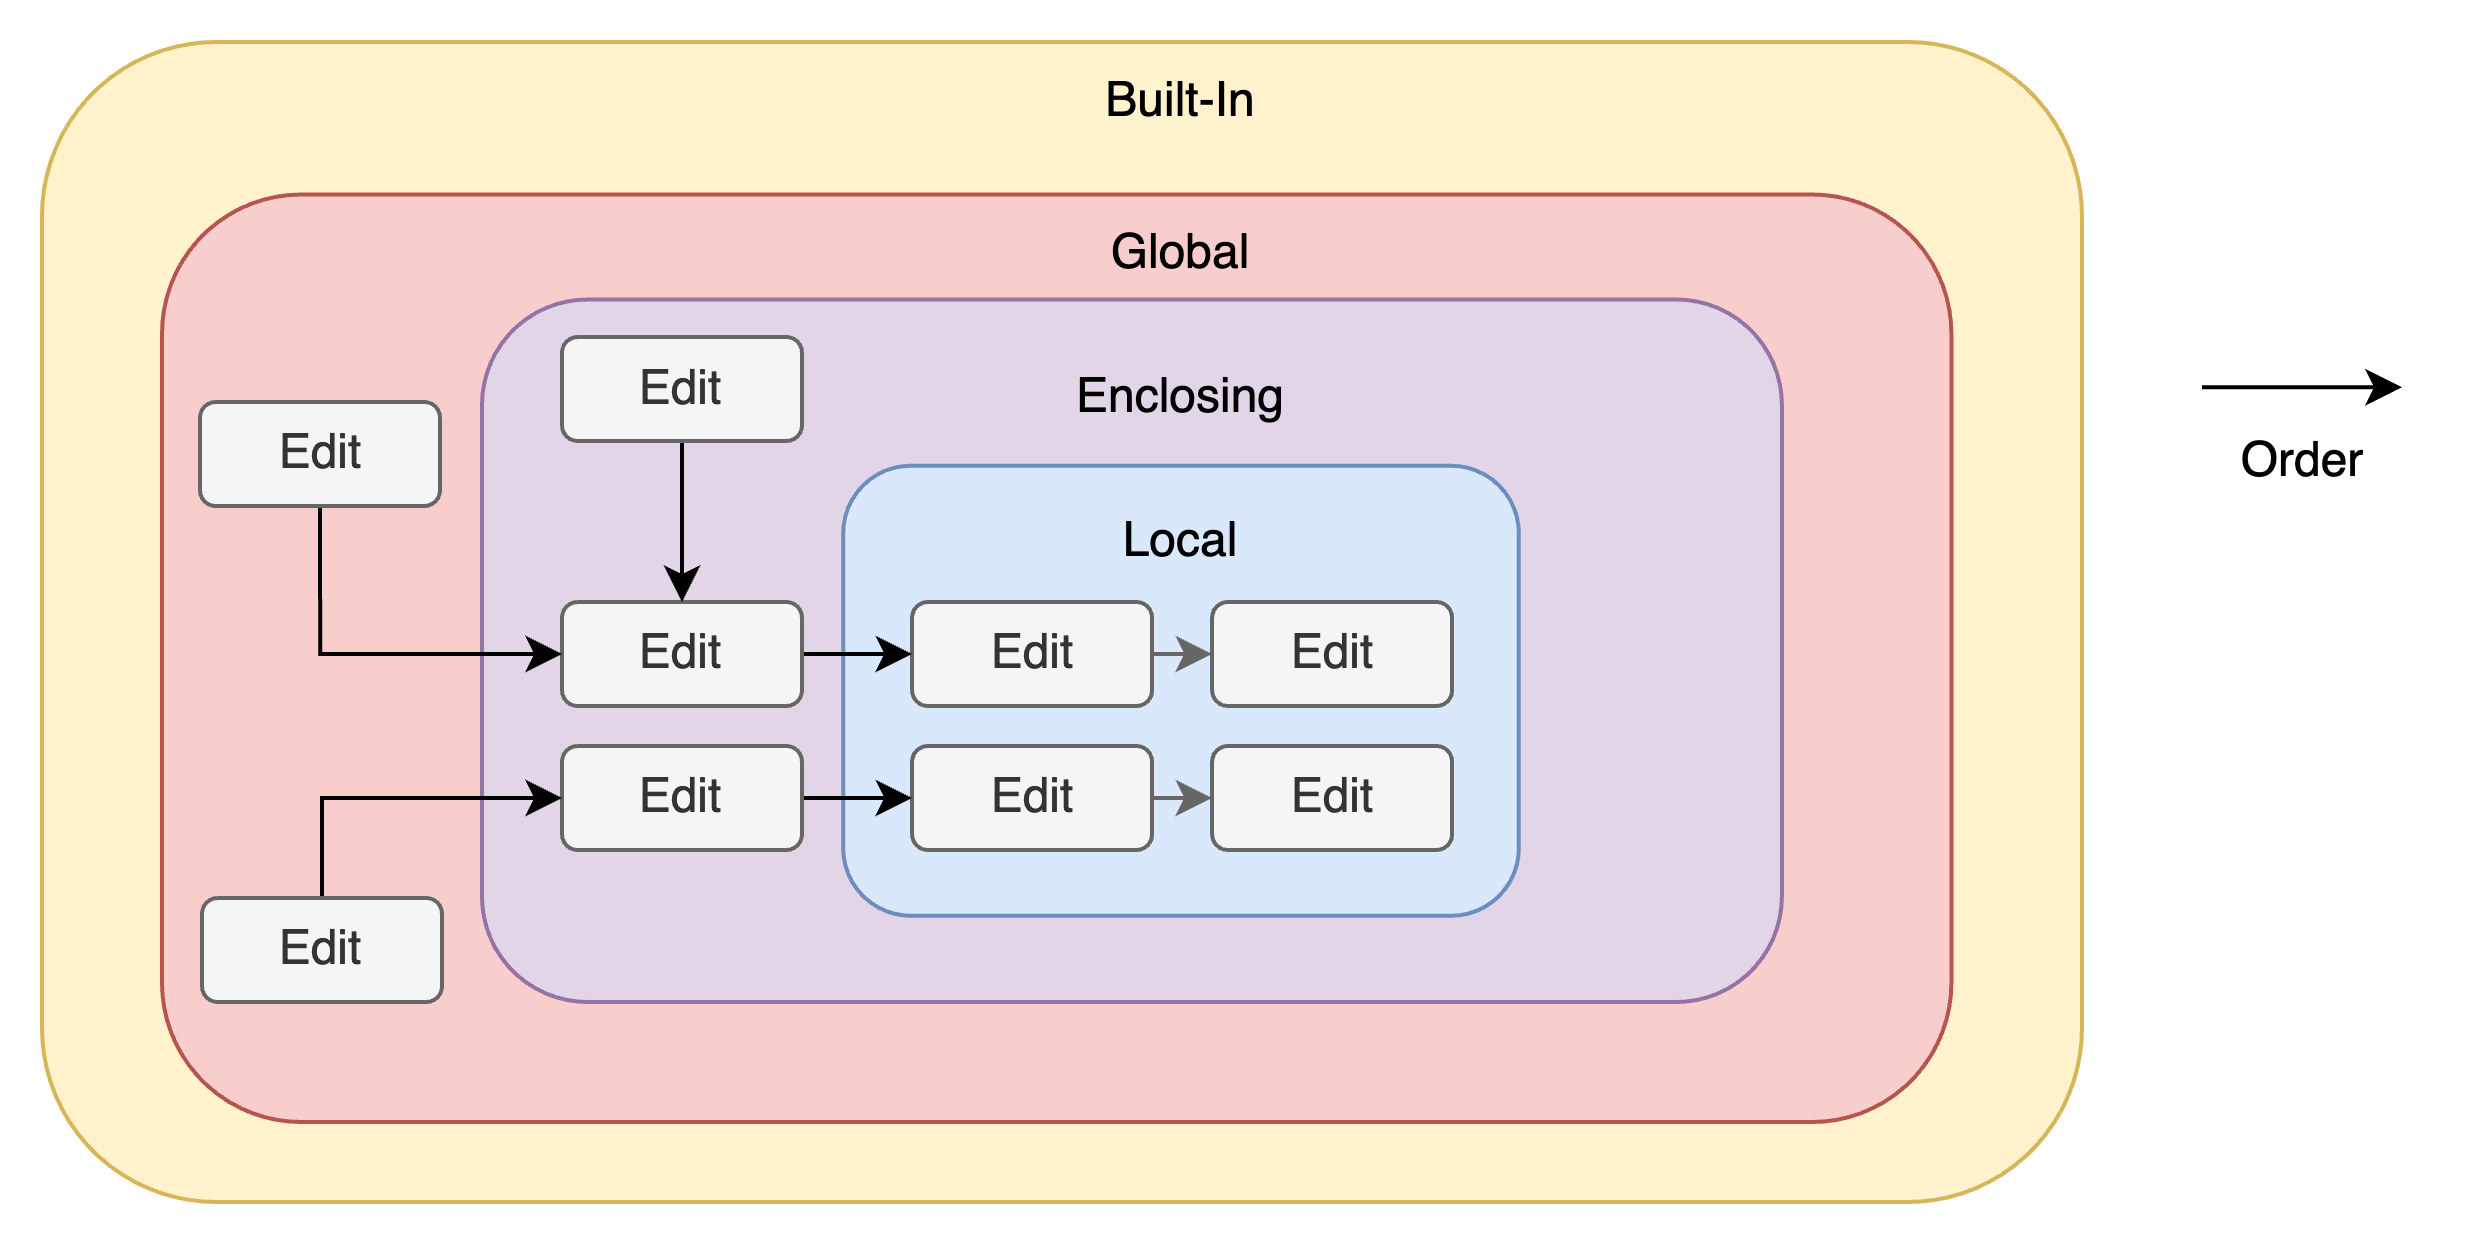
\includegraphics[width=0.6\linewidth]{fig/code_proximity.png}
%     \caption{Code proximity and dependencies}
%     \label{fig:proximity}
% \end{figure}

\subsection{Types of Dependencies}

Given the above observations, we further categorized these edits into three types of dependencies: Syntactic, Semantic, and Proximity. Given two elements \( h_i, h_j \in \mathbf{H} \), the type of relationship between them is defined by a function \( f(h_i, h_j) \) as follows:

\subsubsection{Syntactic Dependency}
Syntactic dependencies arise from structural relationships within the abstract syntax tree (AST). These include:
\begin{itemize}
    \item \textbf{Variable:} Relationships between variable declarations and their usages.
    \item \textbf{Control Flow:} Dependencies introduced by constructs such as loops or conditional statements.
    \item \textbf{Scope:} Relationships governed by scope hierarchies, such as nested blocks or functions.
\end{itemize}
For example, an edit modifying a loop header \( h_i \) might syntactically depend on edits to its body \( h_j \).

\subsubsection{Semantic Dependency}
Semantic dependencies are derived from the meaning and behavior of the code. These include:
\begin{itemize}
    \item \textbf{Type:} Relying on type definitions or changes (e.g., updating function signature affects call sites).
    \item \textbf{Execution Flow:} Relationships influenced by control flow or data flow analysis.
    \item \textbf{Functional Relationships:} Dependencies between a function definition and its invocations.
\end{itemize}
For example, if \( h_i \) modifies a function’s logic and \( h_j \) updates a related test case, they are semantically dependent.

\subsubsection{Proximity Dependency}
Proximity dependencies are based on the physical closeness of edits in the codebase. These dependencies often arise due to:
\begin{itemize}
    \item \textbf{Local Context:} Edits within the same function, class, or block of code.
    \item \textbf{Spatial Relationships:} Edits located near each other in terms of line numbers or columns.
\end{itemize}
For example, two edits \( h_i \) and \( h_j \) that update consecutive lines in the same block likely exhibit a proximity dependency.

\subsubsection{No Dependency}
If \( f(h_i, h_j) = \emptyset \), there is no direct relationship between the edits \( h_i \) and \( h_j \). These edits can be applied independently without affecting the correctness of the codebase.

\subsection{Dependency Matrix Representation}
To facilitate the analysis and visualization of dependencies, we construct a dependency matrix \( D \), where each element \( D_{ij} \) represents the dependency type between \( h_i \) and \( h_j \):
\[
D_{ij} =
\begin{cases}
    \text{1}, & \text{if } f(h_i, h_j) \neq \emptyset \\
    \text{0}, & \text{if } f(h_i, h_j) = \emptyset
\end{cases}
\]
Additionally, the dependency type can be encoded in \( D \) as categorical values, where:
\[
D_{ij} =
\begin{cases}
    \text{S}, & \text{if Syntactic Dependency exists} \\
    \text{M}, & \text{if Semantic Dependency exists} \\
    \text{P}, & \text{if Proximity Dependency exists} \\
    \emptyset, & \text{if no dependency exists.}
\end{cases}
\]
This matrix provides a compact representation of the relationships between edits and serves as input for further analysis or optimization algorithms.


% \subsubsection{Syntactic Dependency}
% A modification in one code segment propagates to other areas that depend on it. If a code segment \( h_i \) is altered and another segment \( h_j \) depends on it, then \( h_j \) may experience compilation or runtime errors if the dependency is not addressed. This type of propagation is directional:
%    \[
%    h_i \rightarrow_{\text{dep}} h_j \text{ if } h_j \text{ has a dependency on } h_i.
%    \]
% \subsubsection{Logical Dependency}
% In cases where a modification in one code segment \( h_i \) requires additional implementation in other segments to fulfill the intended functionality, we define this as logical propagation. This type does not lead to immediate errors but results in incomplete functionality until all related edits are made. Here, \( h_i \) logically precedes \( h_j \):
%    \[
%    h_i \rightarrow_{\text{log}} h_j \text{ if } h_j \text{ logically completes the function of } h_i.
%    \]

% \subsubsection{Semantic Dependency} 

% A modification in one code segment \( h_i \) may influence other segments \( h_j \) with similar code patterns, even if they are not directly related by dependency or logic. These edits share similar semantics, and the propagation is generally applied bidirectionally:
%    \[
%    h_i \leftrightarrow_{\text{sem}} h_j \text{ if } h_i \text{ and } h_j \text{ share semantic similarity and influence each other bi-directionally.}
%    \]


\section{Dependency Derivation}

In this section, different methods were explored and their results were aggregated to estimate the dependency between two different edits, $h_i, h_j \in \mathbf{H}$. 


\subsection{Heuristics}

The heuristic approach leverages observed patterns to establish a relative ordering of edits, denoted as \(\mathbf{H} = \{ h_1, h_2, \dots, h_n \}\). For each edit \( h_i \in \mathbf{H} \), we categorize the edit type (addition, deletion, or modification) and prioritize the ordering based on the following observations:

\begin{enumerate}
\item \textbf{Edit Priority}: Deletions \( h_i \in \mathbf{H}_{\text{del}} \) precede additions \( h_i \in \mathbf{H}_{\text{add}} \). Thus, for any two edits \( h_i, h_j \in \mathbf{H} \), if \( h_i \in \mathbf{H}_{\text{del}} \) and \( h_j \in \mathbf{H}_{\text{add}} \), we have \( h_i \rightarrow h_j \).
\item \textbf{Top-Down Order}: Edits within a single file are applied from top to bottom, yielding an order based on line numbers \( \text{line}(h_i) < \text{line}(h_j) \implies h_i \rightarrow h_j \).
\item \textbf{Import Order}: If \( h_i \) involves a module import and \( h_j \) references it, we establish \( h_i \rightarrow h_j \) based on the dependency.
\item \textbf{Lint Errors:} Procedurally sample across a set of error-free edits \( E = \{e_1, e_2, \dots, e_n\} \) to iteratively construct a valid program \( P = \{p_1, p_2, \dots, p_m\} \), where each intermediate program \( p_j \) is error-free \cite{jimenez2023, pandey2024}.
\item \textbf{Identical Code}: Let $\mathcal{E} = \{e_1, e_2, \dots, e_n\}$ be the set of edits and define $\mathrm{Code}(e_i)$ as the code produced by edit $e_i$. We say that two edits are redundant if 
\[
e_i \sim e_j \quad \Longleftrightarrow \quad \mathrm{Code}(e_i) \equiv \mathrm{Code}(e_j),
\]
where $\equiv$ denotes identical or semantically equivalent code. Merge each equivalence class $[e] = \{e_i \in \mathcal{E} \mid e_i \sim e\}$ into a single representative edit to minimize redundancy and reduce conflicts.
\end{enumerate}


The resultant ordering, \( O_{\text{heuristic}}(\mathbf{H}) \), provides a sequence based on these heuristic rules. 

\subsection{Static Analysis}

The static analysis approach utilizes the set of heuristics identified in the previous section to explicitly identify \textit{possible} dependencies between edits. We define a parser \( P(h_i, h_j) \) to estimate the dependency between two edits \( h_i \) and \( h_j \) by performing the following steps:

\begin{enumerate}
    \item \textbf{Abstract Syntax Tree (AST) Generation:}  
    The parser \( P \) first generates an abstract syntax tree (AST)\footnote{An abstract syntax tree is a tree representation of the syntactic structure of source code, commonly used in compilers and static analysis tools.} (Figure \ref{fig:dependency_graph}) for the source code, capturing structural relationships such as nested blocks, function definitions, and variable declarations.

    \item \textbf{Edit Position and Identifier Extraction:}  
    Using the AST, \( P \) identifies the positions (e.g., line and column numbers) and constructs identifiers\footnote{Identifiers are unique names assigned to variables, functions, or other entities in the code to facilitate tracking and analysis.} for each edit \( h_i \). This information establishes a mapping between the edits and their respective code regions.

    \item \textbf{Dependency Tracing with Language Server Protocol (LSP):}  
    Leveraging the Language Server Protocol (LSP)\footnote{LSP is a protocol standard for language-agnostic static analysis and editor integrations, enabling features like auto-completion, go-to-definition, and dependency tracing.}, the parser traces dependencies by analyzing cross-references, type hierarchies, and function calls between \( h_i \) and \( h_j \). This step captures both local (intra-file) and global (inter-file) dependencies.
\end{enumerate}

\begin{figure}
    \centering
    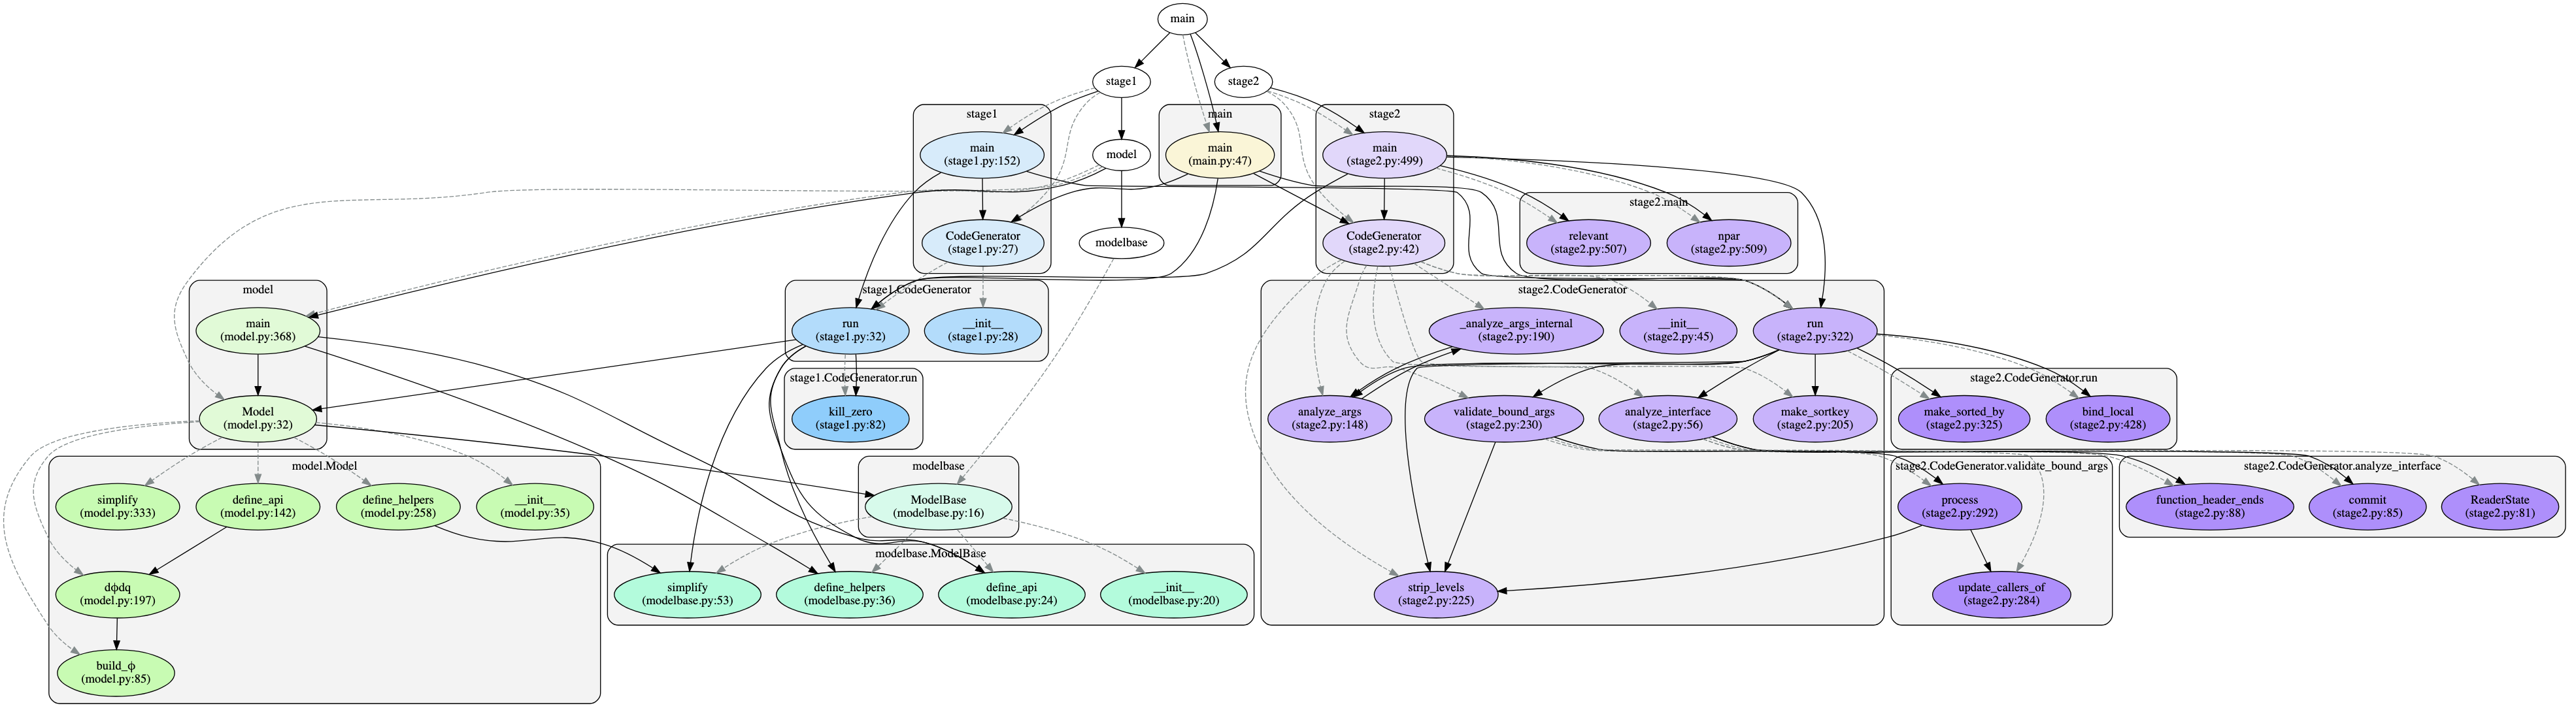
\includegraphics[width=0.8\linewidth]{fig/dependency_graph.png}
    \caption{Pyan constructs a directed graph of the objects in the combined source, and how they define or use each other}
    \label{fig:dependency_graph}
\end{figure}

\subsection{Agents}

The agentic approach uses a language model\footnote{In our experiments, we have mainly adopted GPT4, Gemini-Flash, DeepSeek v3 and Llama.} \( \mathcal{M} \) to infer relationships between edits by providing relevant context for each edit \( h_i \in \mathbf{H} \). For each edit, we create a context vector \( \mathbf{c}(h_i) \), which includes pre-existing code usage data such as function signatures or variable assignments:
\[
\mathbf{c}(h_i) = \{ \text{usage}(h_i), \text{dependencies}(h_i) \}
\]

Given the context vectors \( \mathbf{C} = \{\mathbf{c}(h_1), \mathbf{c}(h_2), \dots, \mathbf{c}(h_n)\} \), the language model \( \mathcal{M} \) attempts to establish a total order:
\[
O_{\text{agentic}}(\mathbf{H}) = \mathcal{M}(\mathbf{C})
\]

This order \( O_{\text{agentic}}(\mathbf{H}) \) reflects the language model's inferred relationships. We will be using Google's Chain of Agents (CoA) framework for multi-agent orchestration.

\section{Context Selection and Prompt Construction}

With limited context\footnote{Although Google's Gemini-Pro has a context window of 2 million token length, we have opted not to use it due to latency and limited hardware.} available, it is not feasible to utilize the entirety of a code repository or external database as input context. To address this limitation, we employ a systematic process to construct the final prompt by selecting the most relevant examples from an external vector database and the repository. This process can be formalized as follows:

\subsubsection{Input Space}
Let \( R \) represent the code repository, consisting of files \( F = \{f_1, f_2, \ldots, f_n\} \), where each file \( f_i \) contains code snippets \( S_i = \{s_{i1}, s_{i2}, \ldots\} \) and comments \( C_i = \{c_{i1}, c_{i2}, \ldots\} \). Additionally, let \( V \) denote the external vector database, consisting of collected examples \( E = \{e_1, e_2, \ldots, e_m\} \), where each example \( e_j \) is a vectorized representation of code snippets or descriptions.

\subsubsection{Relevance Selection Algorithm}
Define a relevance function \( \text{rel}(x, q) \), where \( x \) is a snippet, comment, or vectorized example, and \( q \) is the developer's query or the currently edited code context. The function evaluates the relevance of \( x \) to \( q \). Relevant snippets are selected such that:
\[
S_{\text{rel}} = \{s \in S \mid \text{rel}(s, q) > \tau_s\}, \quad C_{\text{rel}} = \{c \in C \mid \text{rel}(c, q) > \tau_c\}, \quad E_{\text{rel}} = \{e \in E \mid \text{rel}(e, q) > \tau_e\},
\]
where \( \tau_s \), \( \tau_c \), and \( \tau_e \) are predefined thresholds for relevance.

\subsubsection{Ranking}
A ranking function \( \text{rank}(x) \) assigns a priority score\footnote{We experimented with different ranking functions, particularly MSE, MAE etc.} to each selected snippet \( s \in S_{\text{rel}} \), comment \( c \in C_{\text{rel}} \), and example \( e \in E_{\text{rel}} \). The elements are sorted in descending order of their relevance:
\[
\text{rank}(S_{\text{rel}} \cup C_{\text{rel}} \cup E_{\text{rel}}) = \text{sort}\big(S_{\text{rel}} \cup C_{\text{rel}} \cup E_{\text{rel}}, \text{by } \text{rank}(x)\big).
\]

\subsubsection{Filtering}
To ensure the final prompt fits within the context window \( W_{\text{max}} \), a filtering function \( \text{filter}(X, W_{\text{max}}) \) selects the highest-ranked elements from \( X = S_{\text{rel}} \cup C_{\text{rel}} \cup E_{\text{rel}} \) such that:
\[
\sum_{x \in X'} \text{len}(x) \leq W_{\text{max}},
\]
where \( \text{len}(x) \) denotes the token length of \( x \), and \( X' \subseteq X \) is the filtered subset.

\subsubsection{Prompt Assembly}
The final prompt \( P \) is constructed by concatenating the filtered snippets, comments, and examples in their ranked order:
\[
P = \text{concat}(X').
\]

This approach ensures that the final prompt includes the most relevant information from both the repository and the external vector database. The final prompt can be found in Appendix B.
\chapter{Approach}

\section{System Overview}

The overall system design is shown at Figure \ref{fig:overview}.

\begin{figure}[!htb]
    \centering
    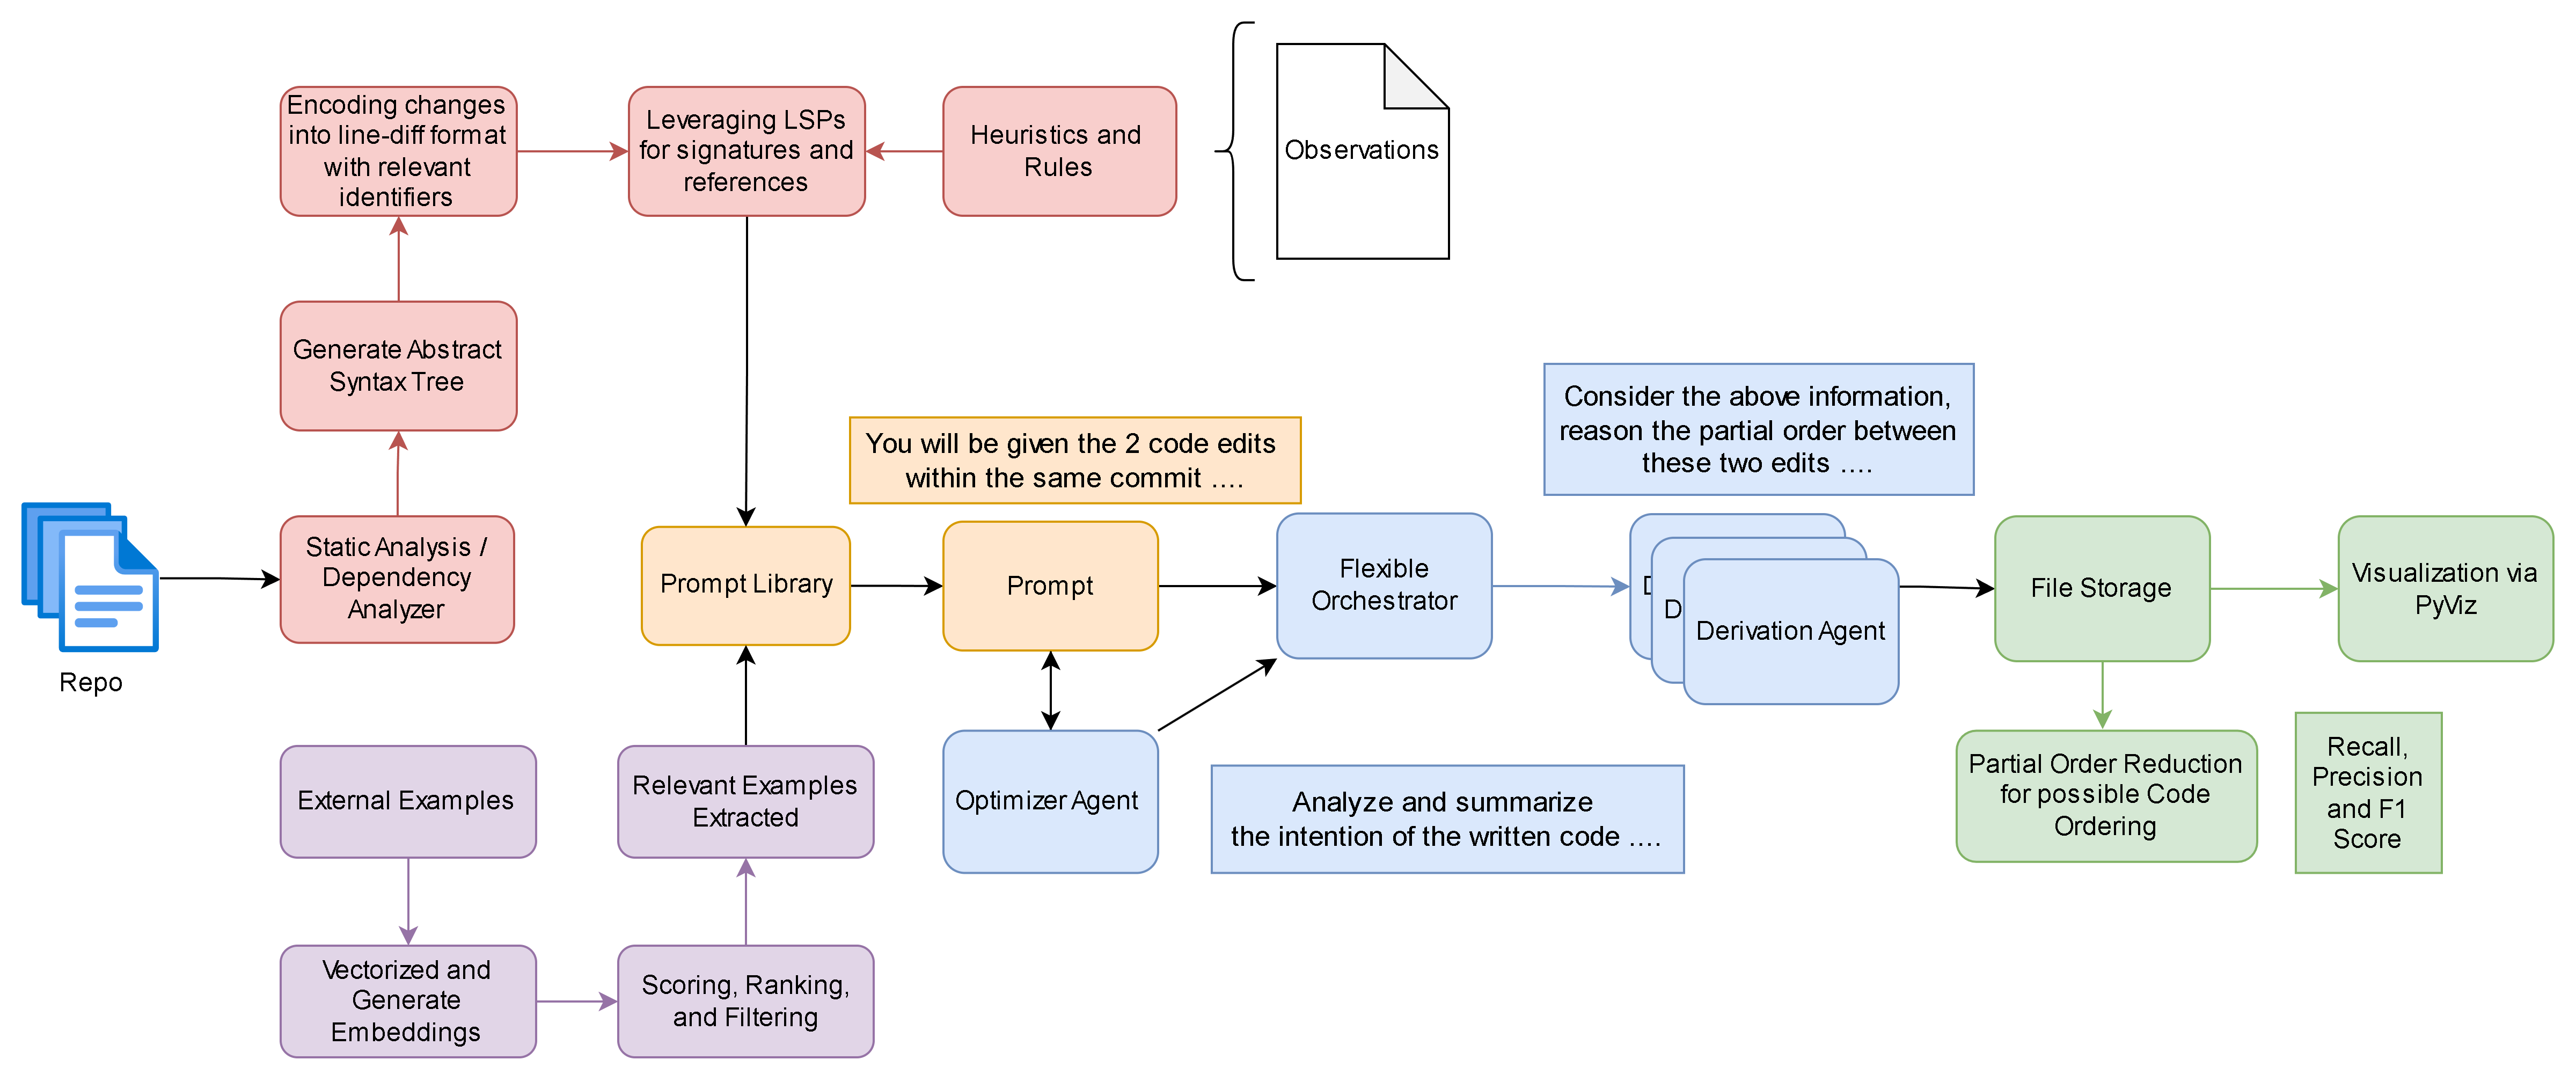
\includegraphics[width=1\linewidth]{fig/overview.png}
    \caption{System Overview}
    \label{fig:overview}
\end{figure}

\section{Encoding Code Changes}

We use a line-diff-based format to encode code changes. Let \( u \) represent a code block composed of lines \( l_1, l_2, \dots, l_m \), with an edit region spanning lines \( l_a \) through \( l_{a+n} \), where \( 1 \leq a \leq a + n \leq m \). For each line \( l_i \) within this range, we associate a status variable \( s_i \) to indicate the type of change applied. The status variable \( s_i \) is defined as follows:

\[
s_i = 
\begin{cases} 
    + & \text{if line \( l_i \) is an addition,} \\
    - & \text{if line \( l_i \) is a deletion,} \\
    = & \text{if line \( l_i \) is unchanged (optional).}
\end{cases}
\]

In addition to line-specific information, each edit region \( R \subseteq u \) is also annotated with contextual metadata, including the file path, denoted as \( p(u) \), and the logic path, denoted as \( \ell(u) \). The logic path \( \ell(u) \) represents the hierarchical structure of the code, encompassing the local block, any enclosing blocks, and the parent block. An example is shown below.

\begin{figure}[h]
\scriptsize
\begin{minted}[breaklines, frame=lines]{python}
--- src/transformers/commands/run.py
+++ src/transformers/commands/run.py

@@61,3 61,1 @@ class RunCommand(BaseTransformersCLICommand): >>>> def register_subcommand(parser: ArgumentParser)

@staticmethod
def register_subcommand(parser: ArgumentParser):
    run_parser = parser.add_parser("run", help="Run a pipeline through the CLI")
-   run_parser.add_argument(
-       "--task", choices=list(SUPPORTED_TASKS.keys()) + list(TTASK_ALIASES.keys()), help="Task to run"
-   )
+   run_parser.add_argument("--task", choices=get_supported_tasks(), help="Task to run")
    run_parser.add_argument("--input", type=str, help="Path to the file to use for inference")
    run_parser.add_argument("--output", type=str, help="Path to the file for writing results post-inference.")
    run_parser.add_argument("--model", type=str, help="Name or path to the model to instantiate.")
\end{minted}
\caption{Encoding code change in src/transformers/commands/run.py}
\label{code:encoded_code_change}
\end{figure}

\begin{figure}
    \centering
    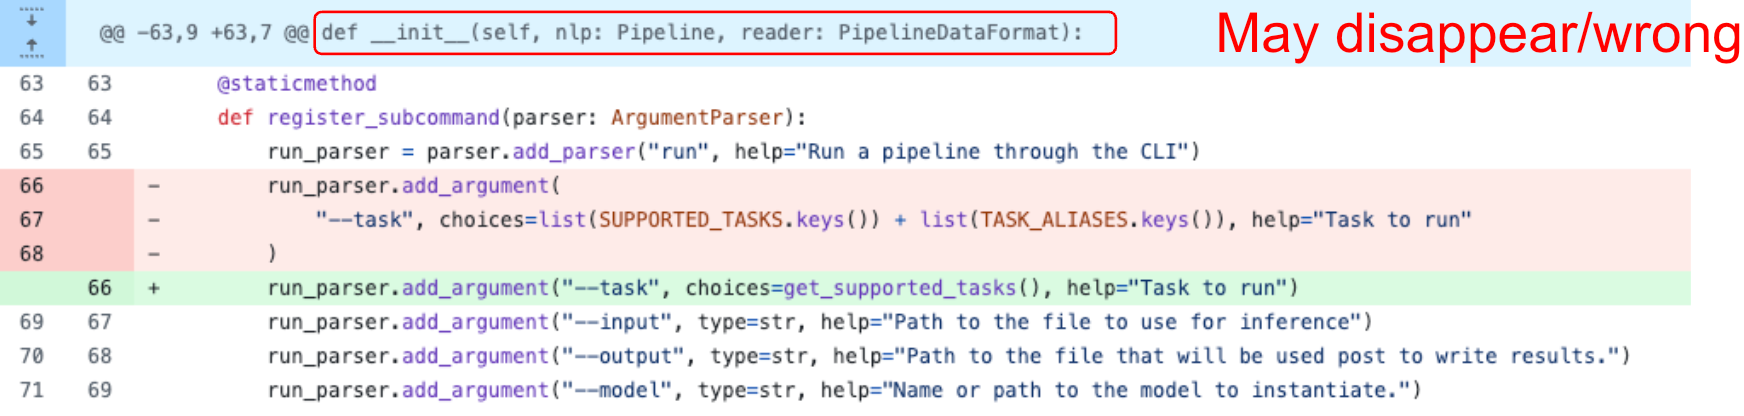
\includegraphics[width=1\linewidth]{fig/encode.png}
    \caption{Original edit span in src/transformers/commands/run.py}
    \label{fig:original_code_change}
\end{figure}

% \section{Analyzing Relevant Signatures}

% With our method for encoding code changes in place, we also need an efficient approach for inputting \( U \), the remaining codebase, into the model. Inputting the entire codebase directly would generate an excessive number of tokens, overwhelming the model’s context window. Instead, we use lightweight static analysis to extract only the most relevant information for context enhancement.

% For each target code region \( u \), we analyze its pre-edit code and compile a list of its usages. For function usages, we extract the function signature; for variables or class members, we retrieve the initial assignment statement. These extracted signatures and usage statements are then concatenated into a single document, serving as supplementary context for the model to interpret dependencies and relationships more accurately.


\section{Multi-Agent Validation}

We define a multi-staged multi-agent system \( \mathcal{A} = \{ A_1, A_2, \dots, A_k \} \), where each agent \( A_i \) is responsible for validating and deducing dependencies for a subset of edit representations \( E_i \subseteq \mathbf{H} \), with \( \mathbf{H} \) being the complete set of edits. Each agent operates independently to analyze the dependencies within its assigned subset \( E_i \) and communicates findings with other agents in the system to achieve consensus on the ordering relationships.

\subsubsection{Stage 1: Optimizer Agent: Information Integration and Summarization}

% In Stage 1, the optimizer agent extracts relevant information in a long-context source and synthesizes relevant information accumulated to generate the response.


% \subsubsection{Stage 2: Worker Agent: Segment Comprehension}

% For each edit representation \( h_j \in E_i \), agent \( A_i \) examines contextual and structural information—encoded as features \( \mathbf{f}(h_j) \)—to determine potential dependencies with other edits \( h_k \in \mathbf{H} \).

% Each agent \( A_i \) thus outputs a set of dependency relationships \( R_i = \{ R(h_j, h_k) \mid h_j, h_k \in E_i \} \), which collectively represent the inferred ordering within its subset. Agents then perform inter-agent validation by communicating these relationships, enabling consensus-building across all subsets \( E_1, E_2, \dots, E_k \). The combined results from all agents form the global dependency graph \( G = (\mathbf{H}, E) \), where \( E \) contains directed edges representing dependencies across all edits.

% By employing a multi-agent approach, this system can efficiently validate complex dependency structures and deduce partial ordering across large sets of edits, enhancing the accuracy and scalability of the ordering inference process.

% \begin{algorithm}
% \caption{Chain of Agents (CoA)}
% \label{alg:coa}
% \begin{algorithmic}[1]
% \Require Source input $x$, query $q$, agent window size $k$, large language model $\text{LLM}(\ast)$.
% \Ensure Answer to the query.
% \State Split $x$ into $l$ chunks $\{c_1, c_2, \dots, c_l\}$ where $c_i$ is shorter than $k$
% \State Initialize $CU_0 \gets$ empty string.
% \For{$i \in \{1,2,\dots,l\}$}
%     \State $CU_i \gets \text{LLM}_{W_i}(I_W, CU_{i-1}, c_i, q)$
% \EndFor
% \State \textbf{return} $\text{LLM}_M(I_M, CU_l, q)$
% \end{algorithmic}
% \end{algorithm}

The optimizer agent operates on the initial set of code edits \( \mathbf{H} \) and aims to condense and structure the available information. Given an input sequence of code modifications, the agent performs the following tasks:

\begin{enumerate}
    \item \textbf{Intent Extraction}: The agent identifies the core intention behind each modification by leveraging large language models (LLMs) to summarize the logical changes, distinguishing between functional enhancements, bug fixes, and refactorings.
    \item \textbf{Pruned Information Output}: Redundant or irrelevant modifications (such as minor formatting changes) are filtered out to ensure a focused summary that retains only information critical to dependency resolution.
\end{enumerate}

Once the optimizer agent has synthesized the high-level description and intention of the code edits, the resulting structured representation is then passed forward to the next stage.

\subsubsection{Stage 2: Segmentation and Distributed Dependency Resolution}

Following the summarization phase, the second stage focuses on decomposing the summarized code changes into smaller, independent segments. This segmentation process is crucial for enabling parallelized dependency analysis across multiple worker agents.

\paragraph{Contextual Segmentation}
The system partitions the summarized code modifications into independent code regions. Given an initial summary \( S \) generated by the optimizer agent, the segmentation module groups the edits into disjoint subsets:
\[
\mathcal{S} = \{ S_1, S_2, \dots, S_n \}, \quad S_i \subseteq S
\]
where each subset \( S_i \) represents a logically independent code fragment. The segmentation criteria are based on:
\begin{itemize}
    \item Scope of the modification (e.g., function, class, or module level)
    \item Interdependencies derived from the call graph and symbol resolution
    \item Heuristic-based clustering using textual and semantic similarity measures
\end{itemize}

\paragraph{Worker Agents: Dependency Inference}
Each segmented context \( S_i \) is independently assigned to a worker agent \( A_i \), which evaluates dependencies between code changes within its assigned context. The dependency inference operates as follows:

\begin{enumerate}
    \item \textbf{Pairwise Comparison}: For each code edit pair \( (e_i, e_j) \in S_i \), the agent determines the relationship \( \mathcal{R}(e_i, e_j) \) by assessing lexical, syntactic, and semantic dependencies.
    \item \textbf{Partial Order Estimation}: The agent constructs a local dependency graph \( G_i \) capturing directed relationships between dependent edits:
    \[
    G_i = (V_i, E_i), \quad \text{where } V_i = S_i \text{ and } E_i = \{ (e_x, e_y) \mid e_x \text{ must precede } e_y \}
    \]
    \item \textbf{Inter-Agent Communication}: Worker agents exchange boundary dependencies where segmented contexts overlap. If an edit \( e_x \) in one subset \( S_a \) influences an edit \( e_y \) in another subset \( S_b \), a cross-agent dependency edge is introduced: \( (e_x, e_y) \in E \).
\end{enumerate}

\paragraph{Dependency Graph Construction}
After all worker agents complete their independent dependency resolution, the local dependency graphs \( G_1, G_2, \dots, G_n \) are aggregated into a global dependency graph:
\[
G = \bigcup_{i=1}^{n} G_i
\]
This final graph encodes the inferred ordering constraints across all code edits, enabling structured application of changes in a manner that preserves logical consistency and correctness.

\subsubsection{Consensus Mechanism and Final Ordering}

To ensure robustness in dependency determination, we introduce a consensus mechanism where conflicting dependencies reported by different agents are reconciled. This is achieved through:

\begin{itemize}
    \item \textbf{Voting-Based Resolution}: If multiple agents provide conflicting orderings for a given edit pair, a majority vote determines the final ordering.
    \item \textbf{Confidence-Weighted Merging}: Dependency edges with higher confidence scores—determined by the strength of inferred relationships—are prioritized.
    \item \textbf{Cycle Detection and Resolution}: The merged dependency graph is checked for cyclic dependencies, which are resolved through a priority-based tie-breaking strategy.
\end{itemize}

The final output of the multi-agent system is an optimized, globally consistent dependency graph that provides a structured execution plan for code modifications.


\chapter{Evaluation}

This evaluation centers on a realistic editing scenario, where we assume that the user has a specific set of code modifications they wish to implement. Our primary objective is to determine how effectively the proposed approach replicates human behavior and intent during these edits. By examining how closely the system’s actions align with typical manual editing patterns, we gain insight into its potential to streamline development workflows and reduce the need for extensive manual intervention.

\section{Dataset}

We construct a dataset of five programming languages (Python, Go, Java, JavaScript, and TypeScript), which consists of 689 most-starred repositories from GitHub,
with 38,197 commits. Dataset statistics are shown in Table \ref{tab:dataset-stats}.

\begin{table}[htbp]
\centering
\begin{tabular}{lcccc}
\hline
\textbf{Language} 
  & \textbf{\# Repositories} 
  & \textbf{\# Commits} 
  & \textbf{\# Edits} \\
\hline
\textbf{Python}      
  & 125   & 8148  
  & 51288 \\

\textbf{Go}          
  & 165   & 7031    
  & 46436 \\

\textbf{Java}        
  & 107   & 13539 
  & 96903 \\

\textbf{JavaScript}  
  & 124   & 2610      
  & 15833 \\

\textbf{TypeScript}  
  & 168  & 7319     
  & 51597\\
\hline
\textbf{Total}       
  & 689 & 38197
  & 257654 \\
\hline
\end{tabular}
\caption{Dataset statistics for each language.}
\label{tab:dataset-stats}
\end{table}

We choose code commits from popular code repositories on GitHub, each of which has a set of edits and a code commit message. The challenges lie in how to construct a dataset which can be representative to real-world software development tasks,  especially when the number of code windows is sufficiently large. In this work, instead of randomly sampling the code windows in a project, we propose a sampling technique for code windows with representative diversity.

\begin{figure}[htbp]
\centering
\begin{tikzpicture}[font=\footnotesize]
%--- TYPE 1 ---
% Make the rectangle wider: (0,0) rectangle (3,2) -> 3 units wide
\draw[dashed, thick] (1.5,0) rectangle (5.5,3);
\node[below] at (3.5,0) {Type 1};
% Widen the red bars accordingly
\fill[red!50] (2,2.3) rectangle (5,1.9);
\fill[red!50] (2,1.1) rectangle (5,0.7);

%--- TYPE 2 ---
% Shift this window to the right and make it also 3 units wide
\draw[dashed, thick] (6.5,0) rectangle (10.5,3);
\node[below] at (8.5,0) {Type 2};
\fill[green!50] (7,1.7) rectangle (10,1.3);
\fill[green!50] (7,1.1) rectangle (10,0.7);

%--- TYPE 3 ---
% Shift further and make it 3 units wide
\draw[dashed, thick] (11.5,0) rectangle (15.5,3);
\node[below] at (13.5,0) {Type 3};
% Top "new version" bar (green)
\fill[green!50] (12,2.3) rectangle (15,1.9);
\fill[green!50] (12,1.7) rectangle (15,1.3);
% Bottom "old version" bar (red)
\fill[red!50]   (12,1.1) rectangle (15,0.7);

%--- LEGEND (optional) ---
\node[draw, dashed, thick, minimum width=0.8cm, minimum height=0.4cm]
      at (1,-1.2) {};
\node[right] at (1.4,-1.2) {Sliding window};

\fill[red!50] (4,-1.4) rectangle (4.5,-1);
\node[right] at (4.5,-1.2) {Old version};

\fill[green!50] (7,-1.4) rectangle (7.5,-1);
\node[right] at (7.5,-1.2) {New version};
\end{tikzpicture}
\caption{Sampling strategy of sliding window with real-world edit dynamic}
\label{fig:dataset}
\end{figure}

We sample three types of code windows from a commit, as shown in Figure \ref{fig:dataset}: 

\begin{itemize}
    \item Type 1: A code window with 1 or more edits that involve only deletion, each edit may be complete or partial, as shown in red in the first window type.
    \item Type 2: A code window with 1 or more edits that involve only addition, each edit may be complete or partial, as shown in green in the second window type.
    \item Type 3: A code window containing a mixed of different types of edits, notably addition, deletion and modification as shown in the third window type.
\end{itemize}

In the dataset, the occurred changes in the code window are informative to refrain from unnecessary recommendations on those areas. We sample the above types with a ratio of 1:1:3. We then further adopt $Llama-3-8B-Instruct$ to filter out commits with messages containing vague instructions or multiple intentions, as these contents hinder the model from establishing proper semantic connection between natural language and code editing. The passed commits have their messages refined for brevity and clarity (e.g., removing pull request IDs or committer emails). Our manual check shows that refined commit messages are more natural as edit descriptions, with redundancy removed.

As a result, the three types of sliding windows can reflect the distribution of real-world editing scenarios in terms of edit label position within the window, edit label quantity and edit dynamics.

\section{Recovering Edit Process}

Following the methodology outlined in Section \ref{sec:por}, our goal is to reconstruct the edit sequence of each commit. Once the pairwise dependencies of edits within a commit have been identified, we introduce a framework for deriving \emph{constrained orderings} of nodes in a Directed Acyclic Graph (DAG). We formalize the notion of topological sorts subject to group-based constraints, as well as a depth-first traversal variant that similarly respects user-defined grouping. We provide detailed algorithms that demonstrate how to compute every possible valid ordering.

\subsection{Preliminaries and Notations}

In some scenarios, \emph{additional grouping constraints} are introduced; these constraints require the algorithm to consider certain subsets of nodes (groups) in a particular sequence. We call the resulting orderings \emph{constrained orderings}.

Let $G = (V, E)$ be a directed acyclic graph (DAG), where
\begin{itemize}
    \item $V = \{1,2,\ldots,n\}$ is the set of $n$ nodes.
    \item $E \subseteq V \times V$ is the set of directed edges.
\end{itemize}
An edge $(u,v) \in E$ means $u$ must appear before $v$ in any valid ordering.  
We denote the \emph{indegree} of a node $v \in V$ by $\text{indegree}(v)$, the number of incoming edges to $v$.

\subsection{Constrained Grouping}
We consider a partition (or covering) of the node set $V$ into $k$ groups: 
\[
  \mathcal{G} = \{G_1, G_2, \dots, G_k\} 
  \quad \text{where} \quad
  \bigcup_{i=1}^{k} G_i = V, 
\]
and each $G_i \subseteq V$. We assume a user-specified \emph{ordering} on these groups, denoted by \\ $(G_{\pi(1)}, G_{\pi(2)}, \dots, G_{\pi(k)})$, where $\pi$ is a permutation of $\{1,2,\ldots,k\}$. 

The overarching idea is to \emph{respect group order} when constructing a node ordering of $V$: we do not move on to $G_{\pi(i+1)}$ before we exhaust possible nodes in $G_{\pi(i)}$, subject to each node's DAG-based indegree conditions.

\subsection{Topological Sorts with Group Constraints}
\label{sec:topo-group}
\begin{algorithm}[H]
\caption{Topological Sort by Group Order}
\label{alg:topological-sorts-by-group}
\begin{algorithmic}[1]
\Require DAG $G=(V,E)$, \text{indegree} map $\text{indegree}(\cdot)$, group order $(G_1, G_2, \dots, G_k)$
\Ensure All constrained topological orderings of $V$

\State Initialize $\text{visited} \gets \varnothing$, $\text{path} \gets []$

\Function{Backtrack}{path, i}
    \If{$|\text{path}| = |V|$}
        \State \textbf{yield} \text{path} \text{ as a valid ordering}
        \State \Return
    \EndIf
    \State $\text{current\_group} \gets G_i$
    \For{\textbf{each} $n$ in $\text{current\_group}$}
        \If{$n \notin \text{visited}$ \textbf{and} $\text{indegree}(n) = 0$}
            \State $\text{visited} \gets \text{visited} \cup \{n\}$
            \State $\text{path}.\text{append}(n)$
            \For{\textbf{each} neighbor $w$ of $n$ in $G$}
                \State $\text{indegree}(w) \gets \text{indegree}(w) - 1$
            \EndFor
            \State \Call{Backtrack}{path, i}
            \For{\textbf{each} neighbor $w$ of $n$}
                \State $\text{indegree}(w) \gets \text{indegree}(w) + 1$
            \EndFor
            \State $\text{path}.\text{pop}()$
            \State $\text{visited} \gets \text{visited} \setminus \{n\}$
        \EndIf
    \EndFor
    \If{$i + 1 < k$}
        \State \Call{Backtrack}{path, i + 1}
    \EndIf
\EndFunction

\State \Call{Backtrack}{[], 0}

\end{algorithmic}
\end{algorithm}

The procedure in Algorithm~\ref{alg:topological-sorts-by-group} 
explores all possible ways to pick a node from the current group $G_i$ whenever that node has $\text{indegree}(n) = 0$. As soon as a node $n$ is chosen, it is appended to the path, and the indegree of its neighbors is decreased. We recursively proceed until the entire node set is exhausted or move on to the next group. Each valid path upon reaching full length is a \emph{constrained topological ordering}.

\subsection{Finding Connected Components (Undirected View)}
Although our graph is a DAG, for some applications, we also need to consider the \emph{undirected} version of $G$, denoted $G^{u} = (V, E^{u})$, where $E^{u} = \{\{u,v\} \mid (u,v)\in E \lor (v,u)\in E\}$. A standard Depth-First Search (DFS) on $G^{u}$ identifies connected components.
\begin{algorithm}[H]
\caption{Connected Components in Undirected Graph}
\label{alg:connected-components}
\begin{algorithmic}[1]
\Require Node set $V$, edge set $E$ (directed; treat as undirected here)
\Ensure All connected components $\{C_1, C_2, \ldots\}$

\State Construct $G^{u} = (V, E^{u})$ where $E^{u}$ is the undirected version of $E$
\State $\text{visited} \gets \varnothing$

\Function{DFS}{u, component}
    \State $\text{visited} \gets \text{visited} \cup \{u\}$
    \State $\text{component}.\text{append}(u)$
    \For{\textbf{each} neighbor $w$ of $u$ in $G^{u}$}
        \If{$w \notin \text{visited}$}
            \State \Call{DFS}{w, component}
        \EndIf
    \EndFor
\EndFunction

\For{\textbf{each} node $v$ in $V$}
    \If{$v \notin \text{visited}$}
        \State $\text{component} \gets []$
        \State \Call{DFS}{v, component}
        \State \textbf{yield} $\text{component}$
    \EndIf
\EndFor
\end{algorithmic}
\end{algorithm}


\subsection{Depth-First Traversal by Group}
\label{sec:dfs-group}
In some cases, rather than enforcing a globally minimal node first policy (as in topological sort), one may wish to run a DFS while still \emph{respecting group constraints}. 
\begin{algorithm}[H]
\caption{Depth-First Traversal by Group}
\label{alg:depth-first-traversal-by-group}
\begin{algorithmic}[1]

\Require DAG \(G = (V,E)\), \(\text{indegree}\) map \(\text{indegree}(\cdot)\), group order \((G_1, \ldots, G_k)\)
\Ensure Constrained depth-first traversals of \(V\)

\Function{FindStartingNodes}{G\_i}
    \State \Return \(\{\,v \in G\_i \mid \text{indegree}(v) = 0\,\}\)
\EndFunction

\Function{DFSCompleteTraversal}{s, G\_i, visited, traversal}
    \State stack \(\gets [\,s\,]\)
    \While{stack is not empty}
        \State \(n \gets \text{stack.pop}()\)
        \If{\(n \notin visited\)}
            \State \(visited \gets visited \cup \{n\}\)
            \State \(\text{traversal.append}(n)\)
            \For{\textbf{each} neighbor \(w\) of \(n\) in \(G\)}
                \If{\(w \notin visited\)}
                    \State \(\text{stack.push}(w)\)
                \EndIf
            \EndFor
        \EndIf
    \EndWhile

    \For{\(m \in \Call{FindStartingNodes}{G\_i}\)}
        \If{\(m \notin visited\)}
            \State \Call{DFSCompleteTraversal}{m, G\_i, visited, traversal}
        \EndIf
    \EndFor
\EndFunction

\State \(S \gets \bigl[\Call{FindStartingNodes}{G_1},\dots,\Call{FindStartingNodes}{G_k}\bigr]\)
\Comment{Set of starting nodes per group}

\For{\((s_1,\dots,s_k) \in \prod_{i=1}^k S_i\)}
    \State \(visited \gets \varnothing\)
    \State \(traversal \gets [\,]\)
    \For{\(i \gets 1 \text{ to } k\)}
        \If{\(s_i \notin visited\)}
            \State \Call{DFSCompleteTraversal}{s_i, G_i, visited, traversal}
        \EndIf
    \EndFor
    \State \textbf{yield} \(traversal\)
\EndFor

\end{algorithmic}
\end{algorithm}


Algorithm~\ref{alg:depth-first-traversal-by-group} shows how we generate all possible DFS-based traversals while forcing the sequence of groups. We collect possible \emph{starting nodes} in each group based on $\text{indegree}$ conditions. The \textbf{product} of these sets of starting nodes yields different ways to initiate a DFS in each group. Then, for each combination of starting nodes, we do a full DFS while ensuring that if further valid starting nodes exist in $G_i$, they are explored before switching to the next group $G_{i+1}$.

\subsection{Enumerating All Constrained Sorts for Every Group Ordering}
We can further iterate over every \emph{permutation} of the groups to find all distinct ways the groups may be arranged:
\[
  \text{Permutations of } (G_1, G_2, \dots, G_k) \;=\; \{\,(G_{\pi(1)}, \dots, G_{\pi(k)}) \;|\; \pi \text{ is any permutation of } \{1,\dots,k\}\}.
\]
\begin{algorithm}[H]
\caption{Constrained Sorts for All Group Orders}
\label{alg:constrained-sorts-all-group-orders}
\begin{algorithmic}[1]

\Require \(G = (V,E)\), \(\text{indegree}\) map \(\text{indegree}(\cdot)\), set of nodes \(V\),
        all permutations \(\{\pi_1,\dots,\pi_M\}\) of group partitions,
        boolean \(\text{topo}\) to switch method
\Ensure All constrained node orderings according to each permutation

\For{\textbf{each} permutation \(\pi_j\)}
    \If{\(\text{topo} = \text{True}\)}
        \State \textbf{yield all} \Call{TopologicalSortsByGroup}{\(G, \text{indegree}, V, \pi_j\)}
    \Else
        \State \textbf{yield all} \Call{DepthFirstTraversalByGroup}{\(G, \text{indegree}, \pi_j\)}
    \EndIf
\EndFor

\end{algorithmic}
\end{algorithm}

We have introduced a framework for deriving \emph{constrained orderings} of nodes in a directed acyclic graph. The two major approaches demonstrated are:
\begin{itemize}
    \item A group-constrained \emph{topological sort}, ensuring that nodes are chosen in zero-indegree fashion \emph{within} each group before moving on.
    \item A group-constrained \emph{DFS} approach, enumerating all ways to initiate a DFS for each group, respecting partial orders.
\end{itemize}
By iterating over all permutations of groups, we obtain the full set of valid orderings. This approach can be specialized for tasks such as constrained scheduling, compilation ordering, or phased execution where partial orders must be respected, but some steps are grouped logically.

\section{Evaluation Workflow}
Let $C = \{\,C^{(1)}, C^{(2)}, \dots, C^{(m)}\} $ be the set of all valid orderings of the ground-truth changes. Given a predicted sequence, $P$, we first check whether $P$ exactly matches any $C^{(i)} \in C$.

If there exists an $i$ such that $P = C^{(i)}$, we consider $P$ a perfect match and assign zero cost.

Otherwise, we compute the minimum number of swaps needed to transform $P$ into each $C^{(i)}$, and select 
$\min_{1 \leq i \leq m} \bigl(\mathrm{MinSwaps}(P, C^{(i)})\bigr)$ as the distance metric. Here, $\mathrm{MinSwaps}(\cdot,\cdot)$ measures the minimum swaps required to reorder one permutation into another (assuming both contain the same elements.


\begin{algorithm}[H]
\caption{Minimum Swaps Between Two Permutations}
\label{alg:min-swaps}
\begin{algorithmic}[1]
\Require Two permutations $p$ and $q$ of length $n$
\Ensure The minimum number of swaps needed to transform $p$ into $q$

\Statex

\State \(\textit{inv} \gets \text{array of length } n\)
\For{\(i \gets 1 \text{ to } n\)}
    \State \(\textit{inv}[\,p[i]\,] \gets i\)
\EndFor

\State \(r \gets \text{array of length } n\)
\For{\(i \gets 1 \text{ to } n\)}
    \State \(r[i] \gets \textit{inv}[\,q[i]\,]\)
\EndFor

\State \(\textit{visited} \gets \text{boolean array of length } n\text{, all } \textbf{false}\)
\State \(\textit{countCycles} \gets 0\)

\For{\(i \gets 1 \text{ to } n\)}
    \If{\(\neg \textit{visited}[i]\)}
        \State \(\textit{countCycles} \gets \textit{countCycles} + 1\)
        \State \(j \gets i\)
        \While{\(\neg \textit{visited}[j]\)}
            \State \(\textit{visited}[j] \gets \textbf{true}\)
            \State \(j \gets r[j]\)
        \EndWhile
    \EndIf
\EndFor

\State \(\textit{minSwaps} \gets n - \textit{countCycles}\)
\State \Return \(\textit{minSwaps}\)

\end{algorithmic}
\end{algorithm}

The evaluation results for Python repositories can be seen below: 

\begin{table}[h!]
\centering
\caption{Comparison of Various Programming Languages}
\label{tab:language-comparison}
\begin{tabular}{@{}lrrrrrrr@{}}
\toprule
\textbf{Language} & \textbf{\# Commits} & \textbf{Perfect Matches} & \textbf{Min Swaps} & \textbf{Max Swaps} & \textbf{Avg} & \textbf{Median} & \textbf{Std Dev} \\ 
\midrule
TypeScript & 103 & 22 & 2  & 26 & 10.2 & 9  & 4.1 \\
Python     &  89 & 19 & 1  & 38 & 12.4 & 11 & 5.2 \\
JavaScript &  67 & 13 & 2  & 16 &  7.8 & 7  & 3.5 \\
Go (Golang)&  56 &  9 & 0  & 20 &  8.9 & 7  & 4.3 \\
Java       & 115 & 27 & 3  & 34 & 14.1 & 13 & 6.0 \\
\bottomrule
\end{tabular}
\end{table}

% \chapter{Plans for next semester}

Next semester, the focus will be on implementing the core components of the project, including multi-agent validation, edit propagation models, and evaluation pipelines. In addition to the technical goals, effective project management practices will be established to ensure timely progress, structured documentation, and streamlined communication.

\section{Technical Implementation Goals}

\subsubsection{Dataset Development and Refinement}

The semester will begin with finalizing and refining a comprehensive dataset specifically tailored for multi-file and propagated code edits. This dataset will serve as the foundation for model training, testing, and evaluation. I plan to iteratively refine the dataset, ensuring it includes diverse examples of code dependencies and propagated changes to enable accurate validation and robust model training.

\subsubsection{Implementation of the Multi-Agent System}

The core technical goal will be to develop the multi-agent system for dependency validation across code edits. Each agent will be programmed to handle specific dependency relationships, such as built-in, global, enclosing, and local (BGEL) dependencies. Agent communication protocols will be implemented to ensure agents reach consensus on dependencies, and their combined outputs will be used to construct a comprehensive dependency graph.

\subsubsection{Directed Acyclic Graph (DAG) for Edit Propagation}

To represent relationships identified by the multi-agent system, I will develop an algorithm to construct a Directed Acyclic Graph (DAG). Each node will represent an edit, and directed edges will denote dependencies, enabling systematic tracking of change propagation across the codebase.

\subsubsection{Evaluation Pipeline Setup}

An automated evaluation pipeline will be developed to support testing the model’s effectiveness in real-world editing scenarios. This pipeline will simulate user actions based on ground-truth changes, enabling evaluation through metrics such as Lines, Levenshtein Distance, and Keystrokes. This workflow will ensure continuous testing, allowing for data-driven improvements to the model.

\section{Project Management}

To ensure that these objectives are met efficiently, a structured project management plan will be established, focusing on task tracking, timeline management, and communication.

\subsubsection{Timeline and Milestone Planning}

The semester will be divided into phases, with each phase targeting specific deliverables:
\begin{itemize}
    \item \textbf{Phase 1}: Dataset finalization and multi-agent system setup.
    \item \textbf{Phase 2}: DAG construction and integration with the multi-agent system.
    \item \textbf{Phase 3}: Evaluation pipeline development and initial testing.
    \item \textbf{Phase 4}: Optimization based on preliminary experiment results.
\end{itemize}

Each phase will have clearly defined milestones, allowing for regular assessments of progress and any needed adjustments.

\subsubsection{Task Management and Tracking}

Task tracking tools, such as Trello or Jira, will be used to break down project components into actionable tasks with specific deadlines. Each task will be assigned priority levels, and progress will be tracked to ensure adherence to the timeline. This structured approach will facilitate efficient time management and maintain focus on high-priority objectives.

\subsubsection{Weekly Checkpoints and Progress Reviews}

To keep the project on track, I will set weekly goals and conduct progress reviews. These checkpoints will involve evaluating completed tasks, assessing upcoming challenges, and adjusting timelines or priorities as needed. This approach will help identify potential bottlenecks early and ensure that corrective actions are taken promptly.

\printbibliography
\appendix
\chapter{Preservation Properties of Partial Order Reduction}

Partial Order Reduction (POR) ensures that certain properties of the system being analyzed are preserved in the reduced state space. In this section, we formally prove the preservation of \textit{safety} and \textit{liveness} properties.

\subsection{Preservation of Safety Properties}

A \textbf{safety property} states that "something bad never happens" during the execution of the system. Formally, a safety property can be expressed as:
\[
\phi_{\text{safety}}: \forall \sigma \in \Sigma, \forall s \in \sigma, \quad s \not\models \text{BadState}
\]
where:
\begin{itemize}
    \item \( \Sigma \) is the set of all possible executions of the system.
    \item \( \sigma \) is a specific execution trace.
    \item \( s \) is a state in the trace \( \sigma \).
    \item \( \text{BadState} \) is the set of states violating the safety property.
\end{itemize}

\textbf{Proof:}
1. POR ensures that for every state \( s \) in the original state space, there exists a corresponding state \( s_{\text{red}} \) in the reduced state space.
\[
\forall s \in S, \exists s_{\text{red}} \in S_{\text{red}}: s \sim s_{\text{red}}
\]
where \( \sim \) denotes equivalence under POR.

2. If \( \phi_{\text{safety}} \) holds in the original state space, it implies:
\[
\forall s \in S, \quad s \not\models \text{BadState}.
\]

3. By the equivalence property of POR:
\[
s_{\text{red}} \sim s \implies s_{\text{red}} \not\models \text{BadState}.
\]

4. Therefore, \( \phi_{\text{safety}} \) also holds in the reduced state space:
\[
\forall s_{\text{red}} \in S_{\text{red}}, \quad s_{\text{red}} \not\models \text{BadState}.
\]

Hence, safety properties are preserved under POR.

\subsection{Preservation of Liveness Properties}

A \textbf{liveness property} states that "something good eventually happens." Formally, a liveness property can be expressed as:
\[
\phi_{\text{liveness}}: \forall \sigma \in \Sigma, \exists s \in \sigma, \quad s \models \text{GoodState}
\]
where \( \text{GoodState} \) is the set of states satisfying the liveness property.

\textbf{Proof:}
1. For liveness properties, POR ensures that every transition in the original state space is represented in the reduced state space. This is guaranteed by the ample set condition:
\[
\forall t \in T, \exists t_{\text{red}} \in T_{\text{red}}: t \sim t_{\text{red}}.
\]

2. Let \( \sigma \in \Sigma \) be an execution trace in the original state space. Since \( \phi_{\text{liveness}} \) holds, there exists a state \( s \in \sigma \) such that:
\[
s \models \text{GoodState}.
\]

3. By POR, every trace \( \sigma_{\text{red}} \in \Sigma_{\text{red}} \) in the reduced state space contains an equivalent state \( s_{\text{red}} \) such that:
\[
s_{\text{red}} \sim s \quad \text{and} \quad s_{\text{red}} \models \text{GoodState}.
\]

4. Thus, \( \phi_{\text{liveness}} \) holds in the reduced state space:
\[
\forall \sigma_{\text{red}} \in \Sigma_{\text{red}}, \exists s_{\text{red}} \in \sigma_{\text{red}}, \quad s_{\text{red}} \models \text{GoodState}.
\]

Hence, liveness properties are preserved under POR.

\subsection{Conclusion}
The preservation of both safety and liveness properties demonstrates that the reduced state space produced by Partial Order Reduction is sound and complete with respect to the properties being verified:
\[
\forall \phi \in \mathcal{P}, \quad (S, T, s_0) \models \phi \iff (S_{\text{red}}, T_{\text{red}}, s_0) \models \phi.
\]
This guarantees that the reduction does not compromise the correctness of the analysis.

\chapter{System Prompt}

\lstset{
    basicstyle=\scriptsize\ttfamily, % Small font size and monospaced font
    breaklines=true,            % Enable line wrapping
    frame=single                % Add a frame around the content
}

\begin{lstlisting}[language=json, basicstyle=\fontsize{8}{10}\selectfont\ttfamily]   
<Task description>
You will be given the 2 code edits within the same commit, analyze what is deleted and added in the 2 edits, and their relationship before and after the edit. Recover the edit scenario and predict their editing order based on the causal relationships. Not all edit pairs have causal relationships.
</Task description>

<Referenceable relationships>
There are several relationships you can refer to:
1. Cut-Paste: A code snippet is removed from one location and placed elsewhere. The cut action typically precedes the paste action.
2. Copy-Paste: Similar code appears in both locations before and after the edits, indicating duplication. This relationship is generally bidirectional.
3. Positional Order: The edits occur close together in the same file (\leq 10 lines apart) and share a similar context, block, or scope.
4. Dependency: A dependency relationship is created or removed between the edits. Ignore this relationship if it already existed in both the pre-edit and post-edit states.
5. Logical Order: Both edits are essential to implement a specific feature and are interdependent.
6. Import-Use: A special case of dependency where one edit involves an import statement, and the other involves the use of the imported symbol. The edit with reference to the method or variable introduced in the import should be the source edit, and the import edit should be the target. 
</Referenceable relationships>

<Response schema>
You must respond in pure JSON format. Ensure the response strictly adheres to the following schema:
{   
    "context": describe if the two edits belong to the same file, scope or block, and if any, affects the relationship between the two edits, Make use of the static information provided.
    "deleted_in_edit_1": describe the deleted code in edit 1,
    "added_in_edit_1": describe the added code in edit 1,
    "deleted_in_edit_2": describe the deleted code in edit 2,
    "added_in_edit_2": describe the added code in edit 2,
    "how_deleted_in_edit_1_and_deleted_in_edit_2_are_related": describe the relationship between the deleted code in edit 1 and the deleted code in edit 2,
    "how_deleted_in_edit_1_and_added_in_edit_2_are_related": describe the relationship between the deleted code in edit 1 and the added code in edit 2,
    "how_added_in_edit_1_and_deleted_in_edit_2_are_related": describe the relationship between the added code in edit 1 and the deleted code in edit 2,
    "how_added_in_edit_1_and_added_in_edit_2_are_related": describe the relationship between the added code in edit 1 and the added code in edit 2,
    "reason": string, // A textual explanation of the rationale.
    "referenced_relationships": list[string] | None, // A list of relevant relationships. You may add your own relationships if applicable.
    "source_edit_idx": 1 | 2, // The index of the source edit
    "target_edit_idx": 1 | 2, // The index of the target edit
    "source_role_in_relationship": string, // Describe how the source edit is involved in the relationship
    "target_role_in_relationship": string, // Describe how the target edit is involved in the relationship
    "causal_direction": string // One of the following: "unidirectional, "no_relation", "bidirectional"
}
</Response schema>

<Response example>
{
    "context": "the two edits are in the same file, but in different block. They are likely to be unrelated.",
    "deleted_in_edit_1": "no deleted code",
    "added_in_edit_1": "add `@total_ordering` Decorator, used to automatically derive comparison methods",
    "deleted_in_edit_2": "delete `__cmp__` method, used in python 2",
    "added_in_edit_2": "updated to method `__lt__` and `__le__`",
    "how_deleted_in_edit_1_and_deleted_in_edit_2_are_related": no relationship,
    "how_deleted_in_edit_1_and_added_in_edit_2_are_related": no relationship,
    "how_added_in_edit_1_and_deleted_in_edit_2_are_related": no relationship,
    "how_added_in_edit_1_and_added_in_edit_2_are_related": `@total_ordering` combines `__lt__` and `__le__` to automatically derive other comparison methods,
    "reason": "Edit 1 add `@total_ordering` Decorator, and Edit 2 replaced method `__cmp__` with `__lt__` and `__le__`. When 2 edits are combined together, the decorator ensures all comparison methods are derived automatically based on the explicitly defined `__lt__` and `__le__`",
    "referenced_relationships": ["Logical order"],
    "source_edit_idx": 1,
    "target_edit_idx": 2,
    "source_role_in_relationship": "Edit 1 is the decorator",
    "target_role_in_relationship": "Edit 2 only implement `__lt__` and `__le__` because of the decorator",
    "causal_direction": "bidirectional"
}
</Response example>


Here is the summary of the code edits:
{hunk1}
{hunk2}

<Static Information>
Use the following information to aid in your decision making.

{dependency_info}
</Static Information>

<Commit Message>
{commit_message}
</Commit Message>

<Commit Summary>
The following anaylsis is made by another AI agent. You may find it helpful to refer to it. 

{summary}
</Commit Summary>

Your response (JSON framework must be constructed with double-quotes. Do not enclose JSON content between ```json and ``` tags).
\end{lstlisting}    

\end{document}